\chapter{Water-saving irrigation can mitigate climate change but entails negative side effects on biodiversity in rice paddy fields}
\markboth{\MakeMarkcase{Chapter 1. Water-saving irrigation can mitigate climate change but entails \\ negative side effects on biodiversity in rice paddy field}}{}
\label{Chapter1}

\begin{center}
\textbf{
Sebastián Echeverría-Progulakis\textsuperscript{1},
Maite Martínez-Eixarch\textsuperscript{1},
Dani Boix\textsuperscript{3}
Raul Llevat\textsuperscript{2}
Lluís Jornet\textsuperscript{1}
Joan Noguerol Arias\textsuperscript{4}
Mar Catala-Forner\textsuperscript{2}
Néstor Pérez-Méndez\textsuperscript{1}
}
\end{center}

\vspace{1ex}

\begin{center}
\textsuperscript{1} IRTA, Marine and Continental Waters Program, La Ràpita, 43540, Catalonia, Spain \\
\textsuperscript{2} IRTA, Sustainable Field Crops Program, Amposta, 43870, Catalonia, Spain  \\
\textsuperscript{3} University of Girona, GRECO, Institute of Aquatic Ecology, Girona, 17003, Catalonia, Spain\\
\textsuperscript{4} IRTA, Sustainability in Biosystems Program, Caldes de Montbui, 08140, Catalonia, Spain
\end{center}
%
%\author[inst1,inst2, ]{Sebastián Echeverría-Progulakis}
%
%\affiliation[inst1]{organization={IRTA, Marine and Continental Waters Program},%Department and Organization
%            city={La Ràpita},
%            postcode={43540}, 
%            state={Catalonia},
%            country={Spain}}
%
%\author[inst1,b]{Maite Martínez-Eixarch}
%\author[inst3,b]{Dani Boix}
%\author[inst2,b]{Raul Llevat}
%\author[inst1,b]{Lluís Jornet}
%\author[inst4,b]{Joan Noguerol Arias}
%\author[inst2,b]{Mar Catala-Forner}
%\author[inst2, ]{Néstor Pérez-Méndez}
%
%\affiliation[inst2]{organization={IRTA, Sustainable Field Crops Program},%Department and Organization 
%            city={Amposta},
%            postcode={43870}, 
%            state={Catalonia},
%            country={Spain}}
%
%\affiliation[inst3]{organization={University of Girona, GRECO, Institute of Aquatic Ecology},%Department and Organization 
%            city={Girona},
%            postcode={17003}, 
%            state={Catalonia},
%            country={Spain}}
%            
%\affiliation[inst4]{organization={IRTA, Sustainability in Biosystems Program},%Department and Organization 
%            city={Caldes de Montbui},
%            postcode={08140}, 
%            state={Catalonia},
%            country={Spain}}
%
%\affiliation[ ]{organization=Corresponding authors:  sebastian.echeverria@irta.cat and nestor.perez@irta.cat}
%
%\affiliation[b]{organization=Contributing authors: maite.martinezeixarch@irta.cat, dani.boix@udg.edu, raul.llevat@irta.cat, lluis.jornet@irta.cat, joan.noguerol@irta.cat and mar.catala@irta.cat}

%\doublespacing - Seba: noted out
%\begin{abstract} - Seba: noted out
\section*{Abstract}
Tackling climate change while enhancing biodiversity without compromising production is a main goal in agricultural management. In rice farming, water-saving irrigation techniques alternative to permanent flooding have been globally adopted to face more severe and frequent droughts and have proven effective in reducing greenhouse gas emissions. Yet potential trade-offs with other global concerning issues such as biodiversity conservation are often overlooked. Here we used a field-scale experiment to compare the effects of water management strategies representing a water use gradient \added[id=SE]{(continuous flooding as the lowest intensity water use management; mid-season drainage (MSD) as medium intensity; and alternate wetting and drying (AWD) as the highest intensity management)} on i) greenhouse gas emissions, ii) the abundance and diversity of freshwater biological communities, and iii) crop yield. \added[id=SE]{While a positive climate change mitigation effect was observed under water-saving practices (92.5\% and 67.3\% methane emission decreases for AWD and MSD, respectively, when compared to continuous flooding), these resulted negative for biodiversity conservation. Even though AWD decreased species richness only at the richness peak, a strong negative effect was observed on the abundance of aquatic organisms (decapods, coleopterans, heteropterans, odonates and amphibians).} \deleted[id=SE]{Methane cumulative emissions decreased 92.5\% under the highest intensity irrigation strategy (alternate wetting and drying, AWD) and 67.3\% with medium intensity management (mid-season drainage, MSD), when compared to continuous flooding. The abundance of aquatic organisms was negatively related to the intensity of tested irrigation strategies, with AWD resulting in the strongest negative impact on decapods, coleopterans, heteropterans, odonates and amphibians. Species richness was 53.0\% and 55.0\% lower for MSD and AWD practices, respectively, in contrast to continuous flooding at the moment of highest richness within the season.} Grain yield decreased 12.9\% with AWD management as opposed to continuous flooding but did not vary under MSD. Even though wider adoption of water-saving strategies might help achieving climate mitigation goals while maintaining yields, negative effects on biodiversity should be addressed to preserve highly diverse communities of aquatic organisms and the broad range of ecosystem services they provide. These results point towards marked trade-offs among different agri-environmental issues, therefore, we advocate for more integrative solutions that account for potential side effects when designing alternative water management plans.\\

%\end{abstract} - Seba: noted out

%\begin{keyword}

\noindent\textbf{Keywords:} Biodiversity conservation; greenhouse gas emissions; paddy rice; water management  %- Seba, included: \noindent\textbf{Keywords:} and replaced all \sep for ;

%\end{keyword} - Seba: noted out

%\end{frontmatter} - Seba: noted out

%\linenumbers - Seba: noted out. This command was used to add line numbers to paper MS.

%\doublespacing - Seba: noted out

\section{Introduction}
\label{sec:intro}

Climate change mitigation and adaptation failure, as well as biodiversity loss and ecosystem collapse, are perceived among the most severe global risks over the next decade \citep{worldeconomicforum.2023}. Furthermore, extreme events attributed to climate change, such as the alternation of severe drought periods and heavy rains, are expected to continue negatively impacting food security due to their adverse effects on agricultural production and yield \citep{fao2022}. The latest Intergovernmental Panel on Climate Change (IPCC) report highlights the interdependence of climate, ecosystems and biodiversity, and food security \citep{IPCC2023}. Despite these interrelations made clear, strategies addressing global change are often disconnected and tend to follow independent courses of action, either focusing on climate change mitigation, biodiversity conservation or sustainable development policies, failing to identify potential outcome conflicts or synergistic measures \citep{arneth2020, rusch2022}. Even though integrative approaches like degraded ecosystem restoration \citep{strassburg2020, temperton2019} and the protection of wetlands and non-forest carbon-rich environments \citep{smith2022} achieve to address multiple challenges simultaneously, some strategies within the recently developed frameworks of Nature-Based Solutions (NBS, \cite{seddon2019}) and Climate-Smart Agriculture (CSA, \cite{tripathi2022}) might result in conflicting outcomes if not well implemented. Among climate change mitigation measures that have been proven to hinder ecosystem biodiversity are large area afforestation \citep{veldman2015} and bioenergy crops \citep{hof2018}, large-scale harvest of logging residues in managed forest landscapes \citep{felton2016} and agriculture intensification through an increased use of agrochemicals and synthetic fertilizers \citep{cohen2021}. Additionally, carelessly designed climate mitigation policies exclusively aiming at achieving the Paris Agreement goal of keeping global warming below 2\degree C, could have negative impacts on food security, foiling the achievement of the UN Sustainable Development Goals (SDG) 2 and 15 of “zero-hunger" and “halt biodiversity loss" by 2030 \citep{fujimori2019}.\\

Agrifood systems, and livelihoods depending on them, face the challenge of sustainably providing sufficient, accessible, affordable, safe and nutritious food under current and projected climate change and biodiversity loss processes \citep{fao2022b}. Rice (\textit{Oryza sativa L.}) is a critical staple food for over 3 billion people and its production has recently reached all-time highs \citep{fao2022a, fao2023}. Rice wetlands are widely recognised for their role on greenhouse gases emissions \citep{mitsch2013, mitsch2018} and as biodiversity hotspots \citep{katayama2019}. Rice production is responsible for the largest agriculture related emissions, particularly regarding methane (CH$_{4}$) \citep{schaefer2016, wang2023} due to the anaerobic decomposition of organic matter under flooded soil conditions \citep{burke1990}. Rice paddy fields are also habitat to a broad range of aquatic organisms, including vertebrates and macroinvertebrates, which are susceptible to changes in irrigation managements that modify water permanence periods \citep{lupi2013}. These organisms play a key role in the provision of different ecosystem services in aquatic systems, such as nutrient cycling, pest control and material translocation, which ultimately improves crop yields \citep{nicholls1998, wallace1996, prather2013}. Therefore, to safeguard biodiversity and crop yield while minimizing the contribution of rice agroecosystems to climate change, mitigation strategies should consider potential trade-offs among these agri-environmental issues.\\

Drought events affecting agricultural production are expected to duplicate their frequency at a global scale during the upcoming century in relation to the 1955-2014 period, driven by higher temperatures and precipitation deficits \citep{feng2023}. Water-saving irrigation methods have been developed as alternatives to conventional continuous flooding, adapting rice production to lower water availability and aiming to reduce unproductive water outflows \citep{tuong2003}. These strategies are mainly based on reducing flooding periods by draining fields at different intensities and frequencies across the growing season \citep{kumar2019alternate}. Allowing aerobic conditions into soils decreases CH$_{4}$ emissions, on one hand, due to methanogenic archaea being strictly anaerobic organisms and, on the other, due to stimulated methanotrophy \citep{sass1992, knowles1993}. The mitigation effect of water-saving irrigation strategies in paddy fields have on decreasing CH$_{4}$ emissions, has been largely identified and described \citep{yan2005, fertitta-roberts2019}. On the contrary, the effects of such strategies on the biodiversity of these agro-ecosystems is less known, as policy makers and social awareness tend to focus mainly in issues concerning climate change mitigation \citep{rusch2022}. Most species inhabiting wetland ecosystems are adapted to temporary drying-out, but some are unable to survive droughts or larger drainage periods \citep{biggs1994, williams1996, williams2000}. Previous studies have already identified contrasting outcomes of rice agriculture policies on climate change mitigation and biodiversity conservation \citep{perez-mendez2022}, suggesting a need for management assessments that consider potential collateral effects on these agri-ecosystems \citep{perez-mendez2022}. Although few previous studies have identified potential negative impacts of water shortening in aquatic organisms \citep{mogi1993, lupi2013, watanabe2013, herring2021}, there is still an important knowledge gap regarding the effect of different water saving strategies on wider groups of organisms and how these effects contrast with those on climate change mitigation and rice yield.\\

Even though large adoption of water-saving practices has been observed across Asia \citep{lampayan2015}, their implementation has been scarce in western rice producing countries, mainly due to farmers' concerns regarding potential negative effects on yields \citep{carrijo2017}. Nevertheless, recent observations have proven a shift towards more frequent and intense droughts in central and western Europe and central North America \citep{masson2021ipcc}, while models project that these trends will persist into the future \citep{berg2018}. Assessing the implementation of water-saving adaptation practices in these regions becomes, therefore, crucial to achieve a more resilient rice production. As evidence pointing towards non-significant yield decreases due to improved water-saving strategies mounts up \citep{linquist2015, martinez-eixarch2021, monaco2021}, their implementation assessment should not only consider agronomic goals but also environmental concerns. The present study aims to quantify the effect of different water-saving irrigation practices on greenhouse gas emission rates, rice-associated aquatic biodiversity and yield to identify and assess synergies and/or trade-offs among these agri-environmental issues. Specifically, we performed a field-scale experiment within the Ebro Delta rice production region (North-East Spain) to analyze the impact of three different irrigation strategies, representing a marked water use gradient (conventional flooding \textgreater\ mid-season drainage \textgreater\ alternate wetting and drying) on i) CH$_{4}$ emissions, diversity and abundance of freshwater fauna (fish, amphibians, decapoda, coleoptera, hemiptera and odonata) and iii) rice yield. The tested hypothesis was that strategies with higher impact reducing water inputs entail contrasting agri-environmental outcomes, having a positive impact from climate change mitigation and adaptation perspectives but affecting negatively the abundance and diversity of aquatic species, when compared to continuously flooded fields. This analysis aims to contribute to the decision making process regarding water management in rice production areas, considering the importance of optimizing water resources, but also that of implementing sustainable ecosystem practices able to optimize potential positive and mitigate possible negative outcomes.

\section{Materials and methods}
\label{sec:meth}

\subsection{Study area}
\label{sec:meth_Site}

A field experiment was conducted through the 2022 rice growing season (May to September) within IRTA Ebro Experimental Station facilities in Amposta, Ebro Delta, Spain (40\degree 42' 30.2" N, 0\degree 37' 56.5" E). The region has a Mediterranean climate with mean annual air temperature of 16.5\degree C, hot summers (mean temperature in July: 25\degree C) and mild winters (mean temperature in December: 9\degree C). Mean annual precipitation is around 550 mm, being October the wettest month (75 mm) and July the driest one (20 mm). Soil texture at the study site is silty clay (49.3\% clay; 49.8\% silt; 6.9\% sand). The experimental station is located at 100 m distance from the Ebro riverbank and 20 km from the river's mouth. The Ebro Delta is one of the largest coastal wetlands in the Mediterranean, with a total area of 320 km$^{2}$ and a coastline of approximately 50 km \citep{rodriguez-santalla2021}. Rice production is the main economic activity in the region, representing 63.0\% of the total area \citep{genua-olmedo2016}. Sites surrounding the study area are rice paddy fields managed under a continuous flooding irrigation system throughout the growing season (May to October), which is the conventional practice in the Ebro Delta region. Rice straw incorporation is the common practice across the region, leading to flooded fields after harvest to assist straw decomposition. From November to December fields are either flooded or left to drain, depending on each farmer's management approach and water availability. After the rice growing season, fields are left fallow through the winter period. Due to its large variety of ecosystems and wildlife abundance, the Ebro Delta is considered a biodiversity hotspot, leading to its protection as a Ramsar site, named as biosphere reserve by UNESCO, enlisted within the Natura 2000 protected sites of the European Union, and recognized as the second most important bird area in Spain \citep{day2006, romagosa2013sustainability, genua-olmedo2016}. 

\subsection{Experimental layout}
\label{sec:meth_Exp}

\begin{figure} [ht]
\captionsetup{justification=justified}
	\centering 
	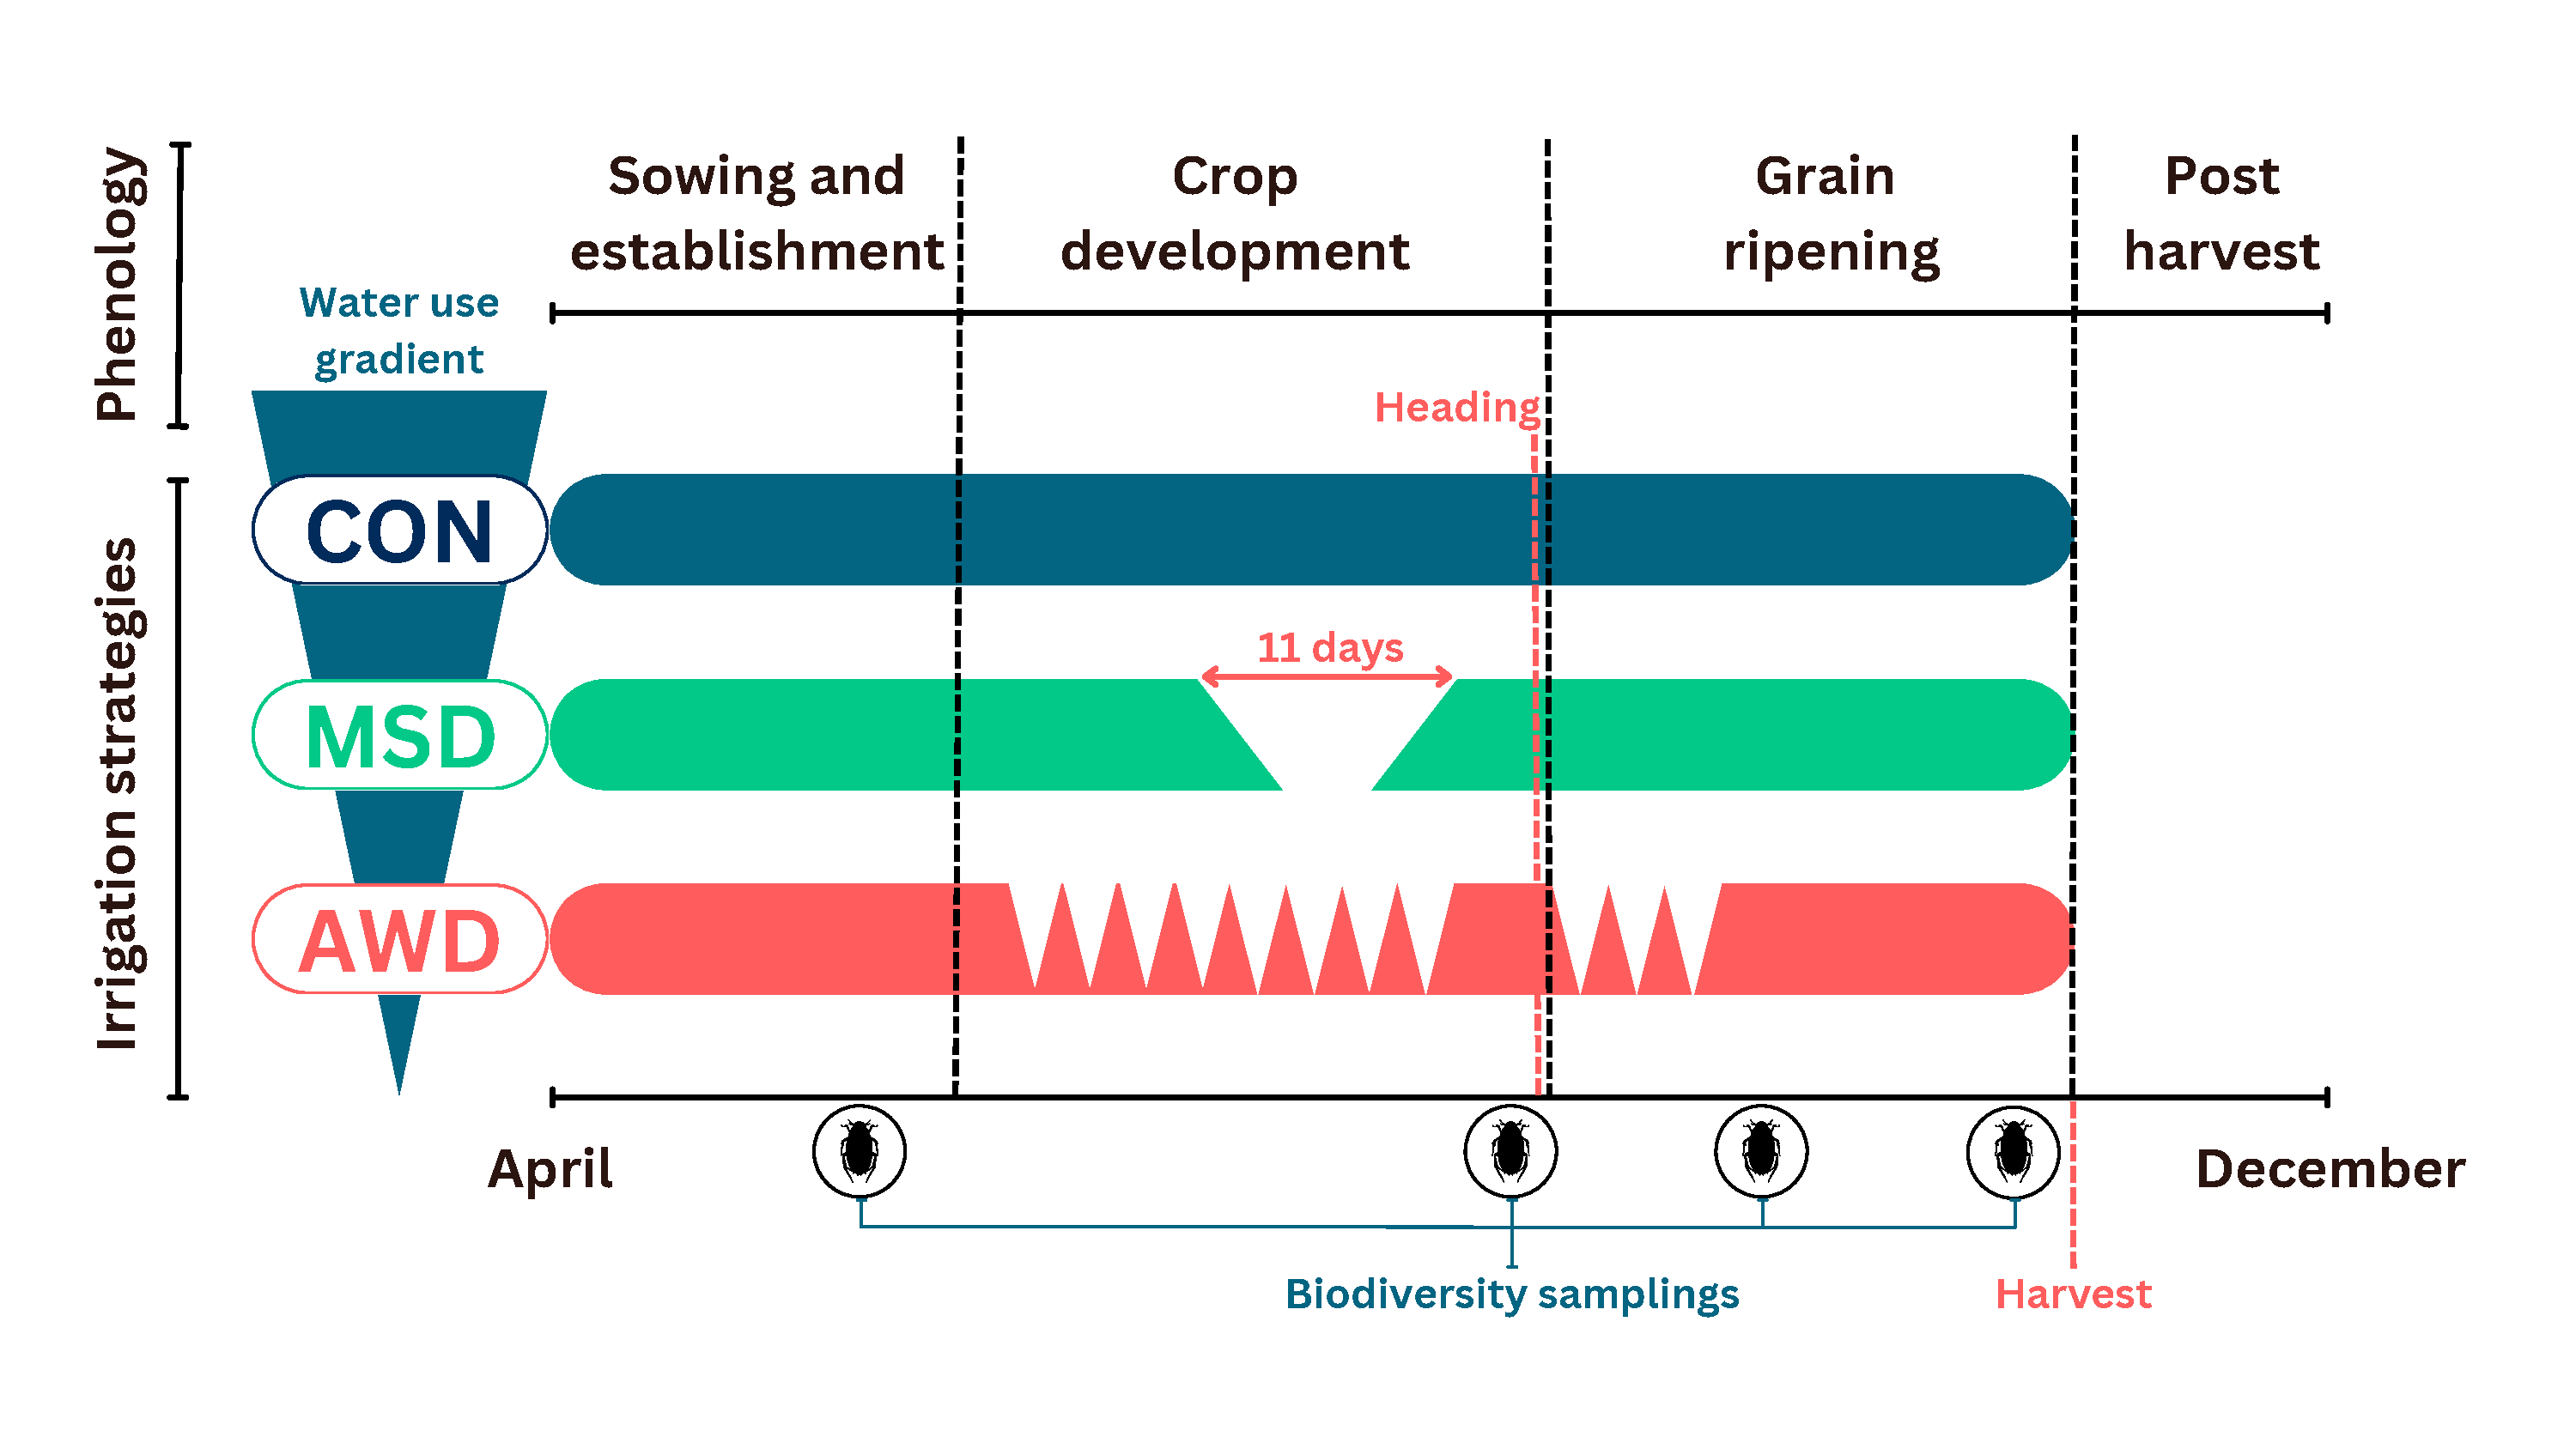
\includegraphics[scale=0.3, center]{Figures/Chapter_1/CERESTRES_Treatments.pdf}
	\captionof{figure}[Treats]{Water-saving irrigation strategies across the water use gradient. Horizontal bars represent reference water layer levels for each strategy through rice phenological stages. Biodiversity sampling dates are also represented across the season. Besides these, weekly greenhouse gas emissions and fortnightly aquatic vertebrate (fish and amphibians) and crayfish abundance samplings were carried out and are not represented in this figure. Abbreviations for assessed irrigation strategies stand for: CON = continuous flooding; MSD = mid-season drainage; and AWD = alternate wetting and drying.}   
	\label{Exp.des}
\end{figure}
%\vspace{0.5cm}\\

Three irrigation practices were tested in a complete randomized block design with five blocks. Each block consisted of three 10 $\times$ 11 m plots, each individually managed under one of the irrigation strategies (Figure \ref{Exp.lay}). Treatments corresponded to tested water-saving irrigation strategies (Figure \ref{Exp.des}): (i) conventional continuous flooding, where plots remained flooded from sowing (May) until two weeks before harvest (September); (ii) mid-season drainage (MSD), draining once, for a 11 days period (from June 30$^{th}$ to July 11$^{th}$, 2022), approximately 20 days before heading; and (iii) alternate wetting and drying (AWD), maintaining fields flooded until 4$^{th}$ leaf stage and from heading to the end of flowering, and under a flooding-drainage cycle through all other periods within the growing season (Table \ref{field_mgmt}). Such flooded periods within the AWD strategy are necessary to avoid physiological stress during emergence, early seedling  and flowering, which are the most sensitive drought-sensitive phenological stages \citep{singh2017developing, yang2019different}. Individual plot management was achieved thanks to independent water inflow and outflow at each plot (Figure \ref{Exp.lay}). Water level was controlled through the installment, and constant monitoring, of piezometers in MSD and AWD plots. AWD is the most widely adopted water-saving irrigation strategy, with reported improved water use efficiency of 18.0-63.0\%, depending on the saturated volumetric water threshold considered for re-flooding, usually termed as AWD severity \citep{linquist2015}. The technique has been improved to minimize yield impacts through the establishment of water table depth thresholds bellow soil surface (usually 15 cm) to trigger field flooding \citep{carrijo2017}, this practice is referred to as Safe-AWD or Mild-AWD. Besides intermittent flooding, MSD was evaluated as a second alternative practice with the objective of establishing a treatment intensity and water use gradient. Treatment intensity is defined by the frequency of dry periods through the growing season. This gradient presents its highest intensity with AWD management (low water use), medium intensity with MSD (medium water use) and lowest intensity with continuous flooding irrigation (high water use). All three treatments followed local conventional practices regarding fertilization, pest and disease control, and straw incorporation. All plots were seeded with JSendra, commercial round rice variety across Spain, and the most prevalent in the Ebro Delta.\\

\begin{table*} [htbp]
    \centering
    \footnotesize  
        \caption{Crop treatments and irrigation management schedule.}
    \begin{tabular}{l l}
\cline{1-2}
{Date} & {Management} \\
\cline{1-2}
%\rule{0pt}{3ex} % inserts space
{10-May-22} & {Fertilization (granulated controlled-release; NPK=33-9-6; 190 kg ha$^{-1}$)} \\
{13-May-22} & {Flooding (all plots)} \\
{17-May-22} & {Sowing (var. JSendra; 500 seeds m$^{-2}$)} \\
{31-May-22} & {Herbicide treatment (Clincher)} \\
{13-Jun-22} & {Start drain-flood cycles in  AWD plots} \\
{30-Jun-22} & {MSD plots drained} \\
{30-Jun-22} & {Herbicide treatment (Logan + Kaos)} \\
{11-Jul-22} & {MSD plots re-flooded} \\
{31-Jul-22} & {Fungicide treatment (Trifloxystrobin)} \\
{11-Aug-22} & {End of drain-flood cycles in  AWD plots} \\
{15-Sep-22} & {Final drain (all plots)} \\
{29-Sep-22} & {Harvest} \\
\cline{1-2}
    \end{tabular}
    \label{field_mgmt}
\end{table*} 


\subsection{Greenhouse gas flux measurement}
\label{sec:meth_GHG}

Gases were sampled through the non-steady state gas chambers method adapted from \cite{martinez-eixarch2018} on a weekly basis from mid-May to late-September 2022. Due to time restrains, samplings were done in three of the total five blocks (i.e., considering three plots per irrigation strategy). Chambers made of polyvinylchloride (PVC) squared frames and covered by transparent plastic were equipped with two ports, sealed with rubber septa, for the insertion of a thermometer and of sampling syringes. The chamber dimensions (129 cm$^{2}$ basal area and 72 cm height) allowed  their installation including several rice plants inside throughout the plant growth, as they were taller than plant height at harvest. Removable foam was set at the base of chambers to allow buoyancy through flooded periods, it was removed when fields were dry. This foam prevented gas exchange between the chamber headspace and the exterior, whereas wet towels were used with this purpose when foam was removed. Chambers were installed and removed for every sampling at the same location within plots. During gas samplings, four gas samples (30 ml) were extracted from each chamber every 10 minutes over a 30-minute period and then transferred over-pressured to pre-evacuated 12 ml vials. Samplings where done consistently from 10:00 to 15:00 to minimize variation derived from daily temperature variability. For every sampling date, soil (electrical conductivity, temperature, redox potential and pH, all measured at 10 cm-depth.) and water (temperature, salinity, oxygen concentration, oxygen saturation and pH) physicochemical parameters were assessed using an automated YSI Professional Plus (Pro Plus) Multiparameter Instrument (Brannum Lane, USA), a Hanna Instruments HI 98190 pH/ORP pH-meter and a Fieldscout direct soil E.C. meter (Spectrum Technologies, 2019). Rice cover (\%) was also recorded during each sampling. CH$_{4}$, CO$_{2}$ and N$_{2}$O concentrations were determined simultaneously using a GC 7820A Agilent (USA) system equipped with a single channel and 2 valves of ten-port gas sampling with back-flush to vent, and 6-port to change between the FID and micro-ECD detectors, using 2 packed columns Hayesep-Q 80-100 mesh 2 m x $1/8''$ x 2.0 mm Ultimetal Agilent (USA), according to \cite{arias2025determination}. The chromatograph calibration was done using CH$_{4}$ standards in nitrogen provided by Carburos Metalicos S.A. (Spain). Temperature variations within headspace of chambers were used to correct gas concentrations according to the ideal gas law. CH$_{4}$ emission rates were calculated as the slope of the linear regression between gas concentration and sampling time. Regressions were considered significant and their slopes accepted as emission rates if they were positive and \textit{R}$^2$ $>$ 0.70, whereas rates below this threshold were considered non-significant linear trends, due to being lower than the method's detection limit or products of ebullition induced by chamber installation, and were given the value of zero \citep{schultz2023}. Besides complete models considering all four measurements per sampling, four alternative models were also assessed, each removing one measurement step-wise and leaving only three remaining measurements. When model requirements were met by the alternative models but not by complete models, the alternative model with higher \textit{R}$^2$ was selected to calculate emissions (calculation example in Figure \ref{mod_exp}). This way, all calculated emission rates considered at least three measurements, the slopes corresponded to those of the best fitting linear models and any potentially altered measurements, due to possible chamber installation issues, were removed from calculations. Seasonal mean cumulative C-CH$_{4}$ emissions (kg ha$^{-1}$) were calculated for each individual plot considering constant rate in between samplings. \\

\subsection{Biodiversity assessment}
\label{sec:meth_BIO}

\replaced[id=SE]{Fish, amphibians and red swamp crayfish}{Aquatic vertebrate (\textit{Carassius carassius}, \textit{Pseudorasbora parva} and \textit{Misgurnus anguillicaudatus} fish species, and \textit{Pelophylax perezi} tadpoles) and red swamp crayfish (\textit{Procambarus clarkii})} communities \added[id=SE]{(Table \ref{AbuMacroFauna})} were characterized sampling individuals fortnightly through the rice growing season installing two cylindrical static nets per flooded plot, identifying to the species level and counting trapped individuals after 24 hours. \added[id=SE]{These samplings were implemented with the objective of capturing the effects irrigation strategies might have on abundance throughout the season, and were later used to compare the resulting cumulative abundance in between strategies across the complete assessed period. }Benthic macroinvertebrate (i.e., different insect groups and juvenile red swamp crayfish) sample collection was carried out separately to fish, amphibians and adult red swamp crayfish using a dip net (250 $\mu$m). Sampled water volume was kept homogeneous by making four net collections across a 30 $\times$ 30 cm plastic frame for each sub-sample. The net was submerged at 1 cm below soil level to collect individuals from the water layer as well as those living just above the soil-water interface. This process was repeated four times per plot and then all collected sub-samples were combined in one recipient, resulting in one final sample per plot. Samples were then washed and stored in 70$\%$ ethyl alcohol for later processing. Macroinvertebrate sample collection was repeated four times through the growing season (June 10$^{th}$, July 15$^{th}$ and August 2$^{nd}$ and 31$^{st}$, 2022) to assess potential changes in community structure and dynamics associated to the irrigation strategies. Sample processing consisted in washing each recipient's content through a 500 $\mu$m mesh sieve and individualizing aquatic organisms (i.e., excluding plant material and terrestrial macroinvertebrates that might have fallen into the traps). Collected organisms were then identified up until the highest possible taxonomic resolution by an experienced taxonomist. Individuals that could only be identified up to a certain level (i.e., order, family or genus), were afterwards assigned to higher levels according to the weighted proportion of individuals in these higher levels.

\subsection{Crop yield}
\label{sec:meth_Yield}

All experimental plots were drained before harvesting to allow machinery entrance. Mechanical harvest was carried out and final yield (kg ha$^{-1}$) was registered per plot to assess potential impacts of water-saving irrigation strategies over production. Yield was calculated as wet weight, immediately after the harvest.  

\subsection{Data analysis}
\label{sec:meth_Stat}

The effect of water-saving strategies on CH$_{4}$ emission rates was analyzed through the application of a generalized linear mixed-modelling (GLMM) approach (model structures are summarized in Table \ref{mod_str}). The CH$_{4}$ emission rate was defined as the dependent variable within models, while the interactions between water-saving strategies and sampling dates were considered as fixed effects (\textit{n} = 213 observations). This interaction was assessed to account for potential temporal variation in the effects of these water regimes on CH$_{4}$ emissions. Soil and water physicochemical parameters were included as covariates within the model after correlation (through Spearman's rank, Figure \ref{Corr_plot}, and Pearson correlation coefficient, Figure \ref{Dendro}) and collinearity (through variance inflation factor, VIF) assessments. Covariates with Pearson's correlation coefficient over 0.75 or VIF over 5 were not included in models. Random effects were accounted for in the model using repetitions (i.e., five replicated blocks) as grouping factor. Gaussian distribution and \textit{identity} link function were applied in the model.\\

The impact of water-saving irrigation strategies on macroinvertebrate communities was evaluated from the perspectives of abundance and diversity. Accumulated abundance (number of total sampled individuals) through the entire rice growing season was assessed for all experimental plots using a subset of the complete biodiversity sampling results. In this, only larvae from water beetles (Coleoptera), water bugs (Hemiptera), dragonflies and damselflies (Odonata) were considered. These three groups were selected in order to work with a single functional group, as they represent the majority of top aquatic predators \citep{lawler2001}. Furthermore, they presented the highest number of species and could be identified to higher taxonomic levels. All individuals in adult stadiums were excluded to avoid potential mobility in between plots, thus focusing the analysis on less mobile individuals more representative of effects on biodiversity due to their higher susceptibility to drainage. Besides these three macroinvertebrate groups, abundance analysis was extended considering decapoda (red swamp crayfish), fish and amphibians (\textit{Pelophylax perezi} tadpoles). Individuals were grouped among orders as maximum taxonomic level to simplify analysis. This first analysis complements posterior diversity analyses, allowing the assessment of any potential effect of irrigation treatments on the amount of individuals per taxonomic level, independent of communities' diversity.  Effects on accumulated abundance of individuals were assessed through a GLM considering abundance as dependent variable and the interaction between irrigation strategy and taxonomic identity as fixed effects (Table \ref{mod_str}). No additional covariates were considered.\\ 

Effects on the diversity of these communities were analyzed considering only macroinvertebrates from the same taxonomic subset as for the abundance analysis. Decapoda, fish and amphibians were excluded due to being composed only by one (i.e., decapoda and amphibians) or very few species (i.e., fish) and, therefore, not representing potential diversity variations. Species richness (\textit{q$_{0}$}) and Shannon diversity (the exponential of  Shannon index, or \textit{q$_{1}$}) for each experimental plot were estimated using the iNext R package (Hill numbers; \cite{chao2014a, hsieh2016}). Both estimations characterize biodiversity profiles within rice fields, species richness indicates the total number of observed species and Shannon diversity can be interpreted as the effective number of common or typical species in the community \citep{chao2014}. Data analysis was done using GLMMs considering biodiversity indexes (\textit{q$_{0}$} and \textit{q$_{1}$}) as each model's dependent variable, the interaction between irrigation strategies and the square of sampling dates as fixed effects, and blocks to account for random effects. A quadratic relation was identified between both biodiversity indexes and sampling date, therefore, the square of sampling (sampling 1 to 4) was included in the model. Soil and water physicochemical parameters were included as covariates after checking for correlation and collinearity, under the same criteria as for CH$_{4}$ emission analysis. For Shannon diversity, a strong interaction was observed between conductivity and water strategies (Figure \ref{vars_Treat}), so it was removed from the model as an explanatory variable to avoid artifacts and isolate the treatments' effect. All abundance and biodiversity models used Gaussian distribution and \textit{identity} link function. Crop yield variations among the assessed strategies were analyzed fitting a linear model considering yield and irrigation treatment as dependent and independent variables, respectively.\\

Data management, visualization and analysis was carried out using R software (R-4.2.2). GLMMs were fit using the \textit{glmmTMB} package \citep{brooks2017}. All models were analyzed through residual diagnostics and R$^{2}$, collinearity and singularity analyses using the \textit{DHARMa} \citep{hartig2018dharma} and \textit{performance} \citep{ludecke2021} R packages, respectively. Analyses of variance (ANOVA) were carried out for all models to identify significant effects. For all cases where different effects were contrasted for factor levels, the \textit{emmeans} package was used \citep{lenth2017}.  

\section{Results}
\label{sec:results}

\subsection{Climate change mitigation} 

Irrigation strategies had a significant effect on C-CH$_{4}$ emission rates ($\chi^2$=59.3, \textit{p}=$<$0.001; Figure \ref{CH4_acc}; results for all ANOVA tests are summarized in Table \ref{mod_res}). Lower rates were identified for both non-continuous irrigation treatments, MSD (\textit{t}=-6.7, \textit{p}=$<$0.001, results for all estimated marginal means paired comparisons are summarized in Table \ref{mod_pairs}) and AWD (\textit{t}=-6.5, \textit{p}=$<$0.001), when compared to conventionally flooded plots. There is high variation among rates from different irrigation managements across the season, evidenced by the significant interaction between irrigation strategies and sampling dates ($\chi^2$=64.8, \textit{p}=$<$0.001). No soil or water physicochemical parameter showed significant effects on emission rates. Considering the overall seasonal emission rate mean, MSD and AWD strategies achieved 69.0\% and 94.0\% decrease in CH$_{4}$ emission rates, respectively, when compared to continuous flooding strategy (continuous flooding = 2.2 $\pm$ 0.3 mg m$^{-2}$ h$^{-1}$; MSD = 0.7 $\pm$ 0.1 mg m$^{-2}$ h$^{-1}$; AWD = 0.1 $\pm$ 0.003 mg m$^{-2}$ h$^{-1}$). Mean cumulative C-CH$_{4}$ emissions for the whole growing season were 64.2 kg ha$^{-1}$, 21.0 kg ha$^{-1}$ and 4.8 kg ha$^{-1}$ for plots managed under continuous flooding, MSD and AWD strategies, respectively. Emissions from non-continuous flooding plots were reduced in 67.3\% with MSD strategy and in 92.5\% with AWD management, when comparing to continuous flooding plots.\\ 

\begin{figure} [ht]
\captionsetup{justification=justified}
	\centering 
	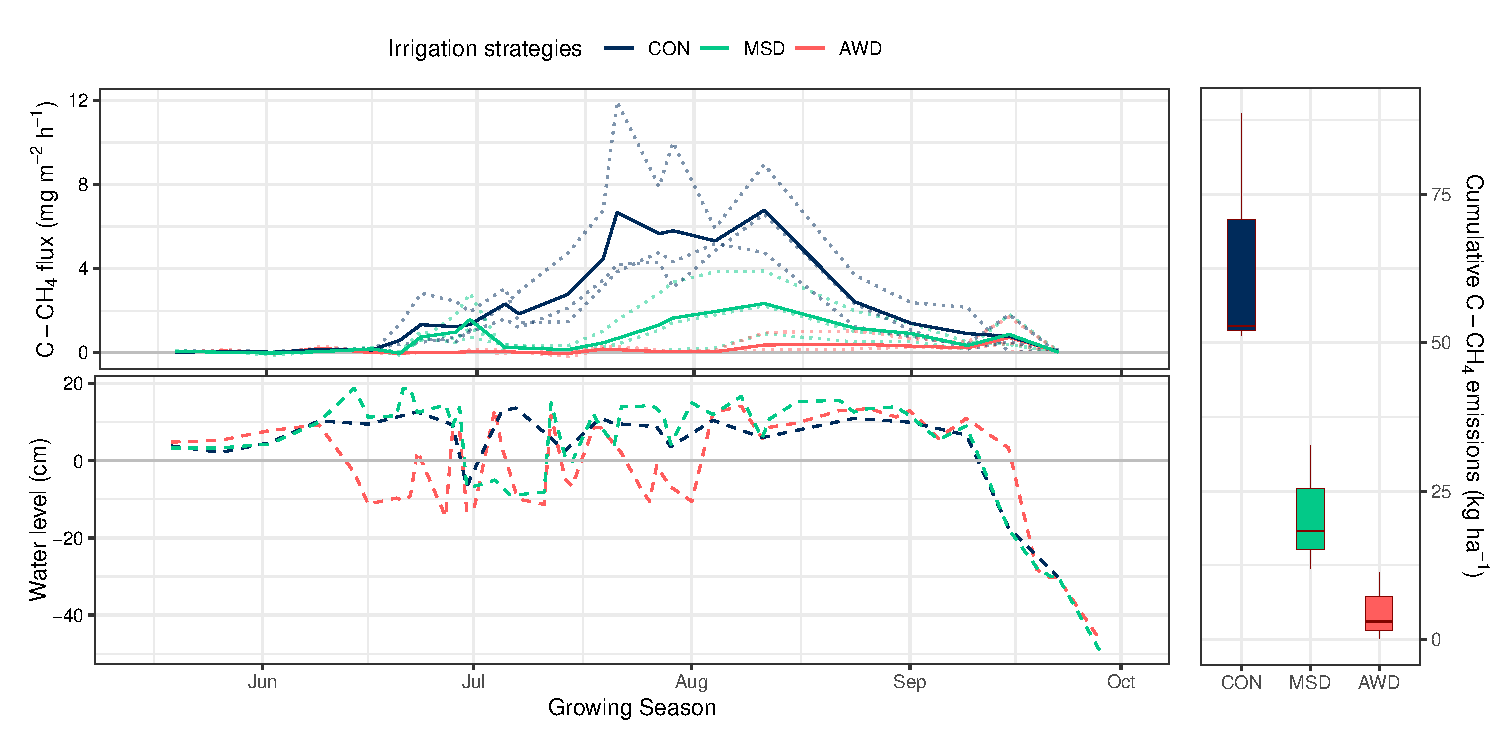
\includegraphics[scale=0.65, center]{Figures/Chapter_1/CH4_flux_water_acc.pdf}
	\captionof{figure}[CH4]{Methane (C-CH$_{4}$) emission rates (top-left panel, in mg m$^{-2}$ h$^{-1}$) and water level (bottom-left panel, in cm) across the rice growing season for the three water-saving irrigation strategies. Discontinuous lines in the top-left panel are mean emissions per plot, continuous lines are treatment means. Right panel shows cumulative C-CH$_{4}$ emissions in kg ha$^{-1}$ for the  rice growing season. Abbreviations for assessed irrigation strategies stand for: CON = continuous flooding; MSD = mid-season drainage; and AWD = alternate wetting and drying.}  
	\label{CH4_acc}
\end{figure}
%\vspace{0.5cm}

\subsection{Biodiversity conservation} 

 Significant differences were identified among irrigation strategies regarding accumulated abundance of vertebrate and macroinvertebrate individuals across the growing season ($\chi^2$=53.2, \textit{p}=$<$0.001), yet a significant statistical interaction between irrigation strategies and taxonomic groups was observed ($\chi^2$=46.2, \textit{p}=$<$0.001). An overall decrease in abundance was observed for AWD plots when compared to continuously flooded plots for most of the assessed taxonomic groups, except for coleoptera and fish (Figures \ref{Abu} and \ref{Abu_date}; and Tables \ref{AbuColOdoHet} and \ref{AbuMacroFauna}). The most extreme effect was observed for amphibians, where abundance tended towards zero values within AWD plots, hindering variance analysis among the three strategies. When re-modelling for a data subset consisting only of amphibian individuals and excluding AWD plots, no difference was identified between MSD and continuous flooding ($\chi^2$=0.3, \textit{p}=0.586). For most groups of aquatic organisms, intermediate abundance levels were achieved by MSD managed plots when compared to continuous flooding and AWD strategies (Figure \ref{Abu}).\\

\begin{figure} [ht]
\captionsetup{justification=justified}
	\centering 
	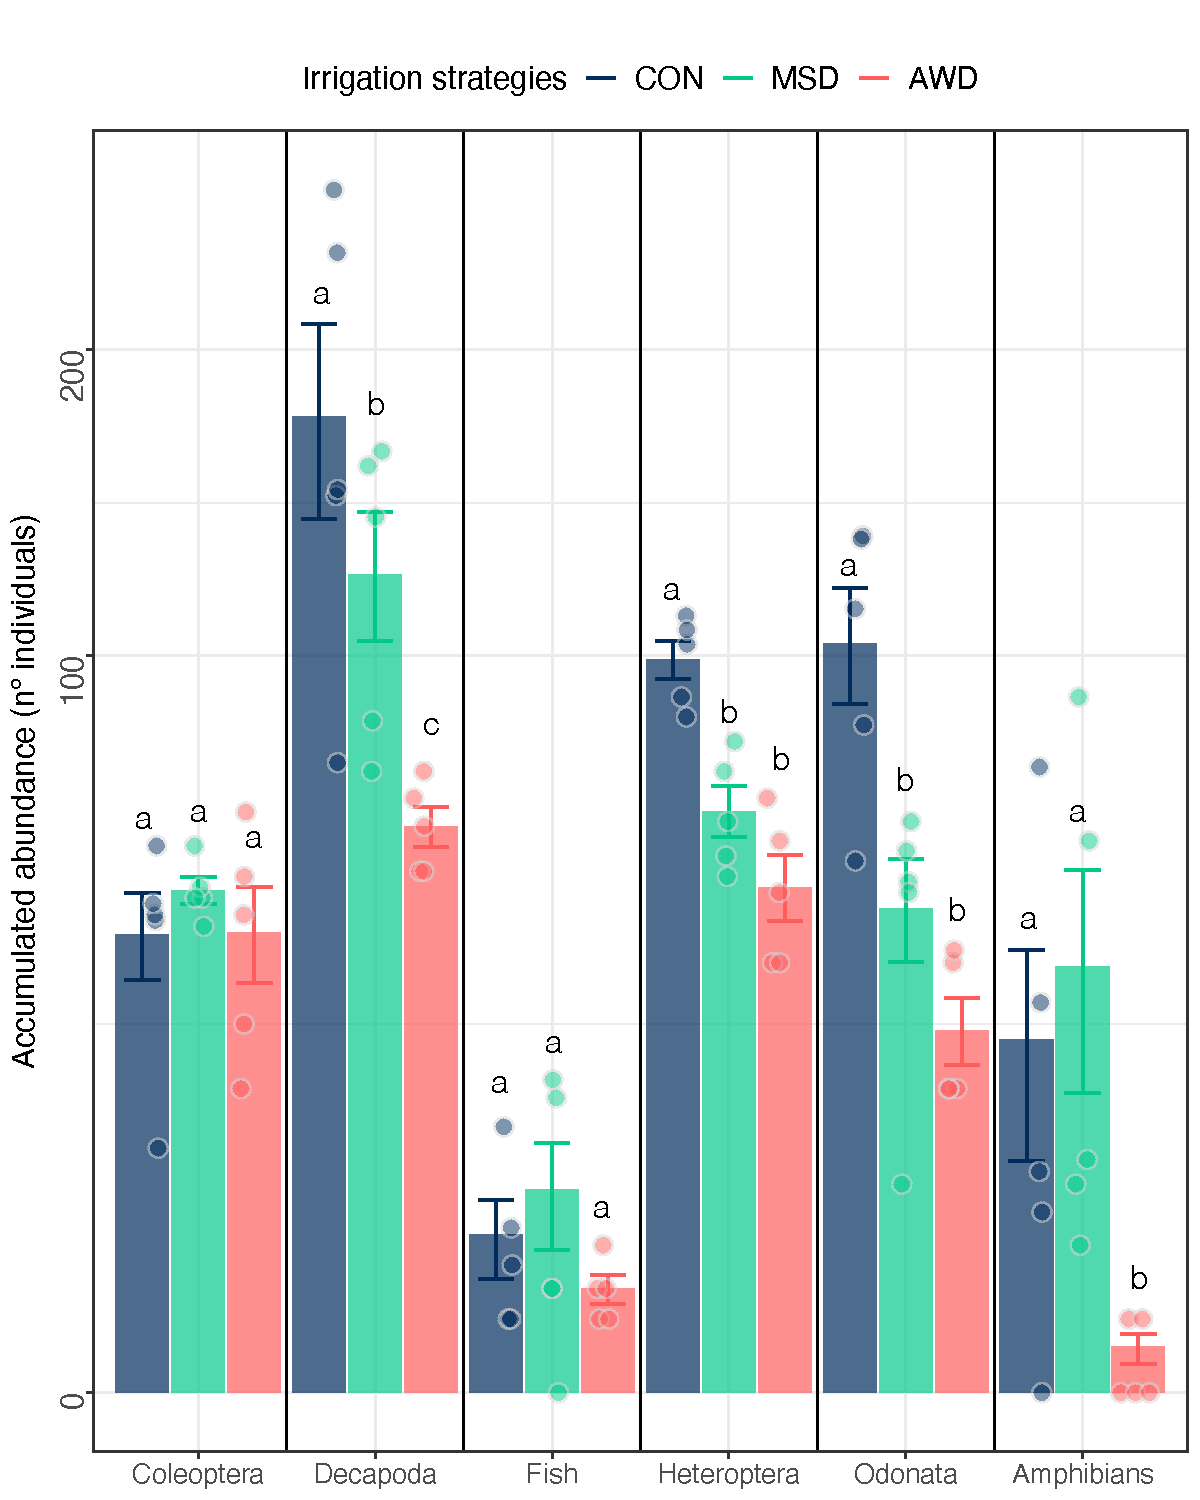
\includegraphics[scale=0.4, center]{Figures/Chapter_1/Abu.div_2022_avg_plots.9.pdf}
	\captionof{figure}[Abundance]{Accumulated abundance (number of individuals) of sampled macroinvertebrates, amphibians and fish for the three water-saving strategies across the rice growing season. Each bar shows the averaged abundance for all samplings and plots according to each strategy, points are abundance results per plot for each sampling and error bars indicate standard errors. Letters above bars show significant statistical differences among irrigation strategies. Abbreviations for assessed irrigation strategies stand for: CON = continuous flooding; MSD = mid-season drainage; and AWD = alternate wetting and drying.}   
	\label{Abu}
\end{figure}
%\vspace{0.5cm}

 Irrigation strategies did not have an overall effect on species richness of aquatic macroinvertebrates ($\chi^2$=3.6, \textit{p}=0.167; Figure \ref{Div_q0}a), but significant effects were observed for the interaction between strategies and the squared sampling dates ($\chi^2$=6.3, \textit{p}=0.043). Covariates with significant effect were the squared sampling dates ($\chi^2$=10.0, \textit{p}=0.002), sampling dates ($\chi^2$=6.6, \textit{p}=0.010), soil electrical conductivity (EC, in $\mu$S $cm^{-1}$; $\chi^2$=6.5, \textit{p}=0.010) and oxygen concentration in the water layer ($O_{2}\%$; $\chi^2$=5.4, \textit{p}=0.020). To further analyze the effect of sampling dates, the effect of irrigation strategies was studied for each independent sampling date, fitting individual GLMMs per each sampling date. A significant effect of irrigation strategy over species richness was identified for the second sampling date ($\chi^2$=71.6, \textit{p}=$<$0.001), but no such effect was evident for all other sampling dates (Figure \ref{Div_q0}b). Within this second sampling, both MSD (\textit{t}=7.1, \textit{p}=$<$0.001) and AWD (\textit{t}=7.8, \textit{p}=$<$0.001) strategies decreased species richness significantly compared to continuous flooding. During this second sampling, MSD and AWD strategies reduced average species richness by 53.0\% and 55.0\%, respectively, versus conventional flooding (continuous flooding = 9.8 $\pm$ 0.7; MSD = 4.6 $\pm$ 0.8; AWD = 4.4 $\pm$ 0.05). Soil pH showed a significant effect ($\chi^2$=11.1, \textit{p}=$<$0.001) on species richness for sampling 2.\\
 
 \begin{figure} [ht]
\captionsetup{justification=justified}
	\centering 
	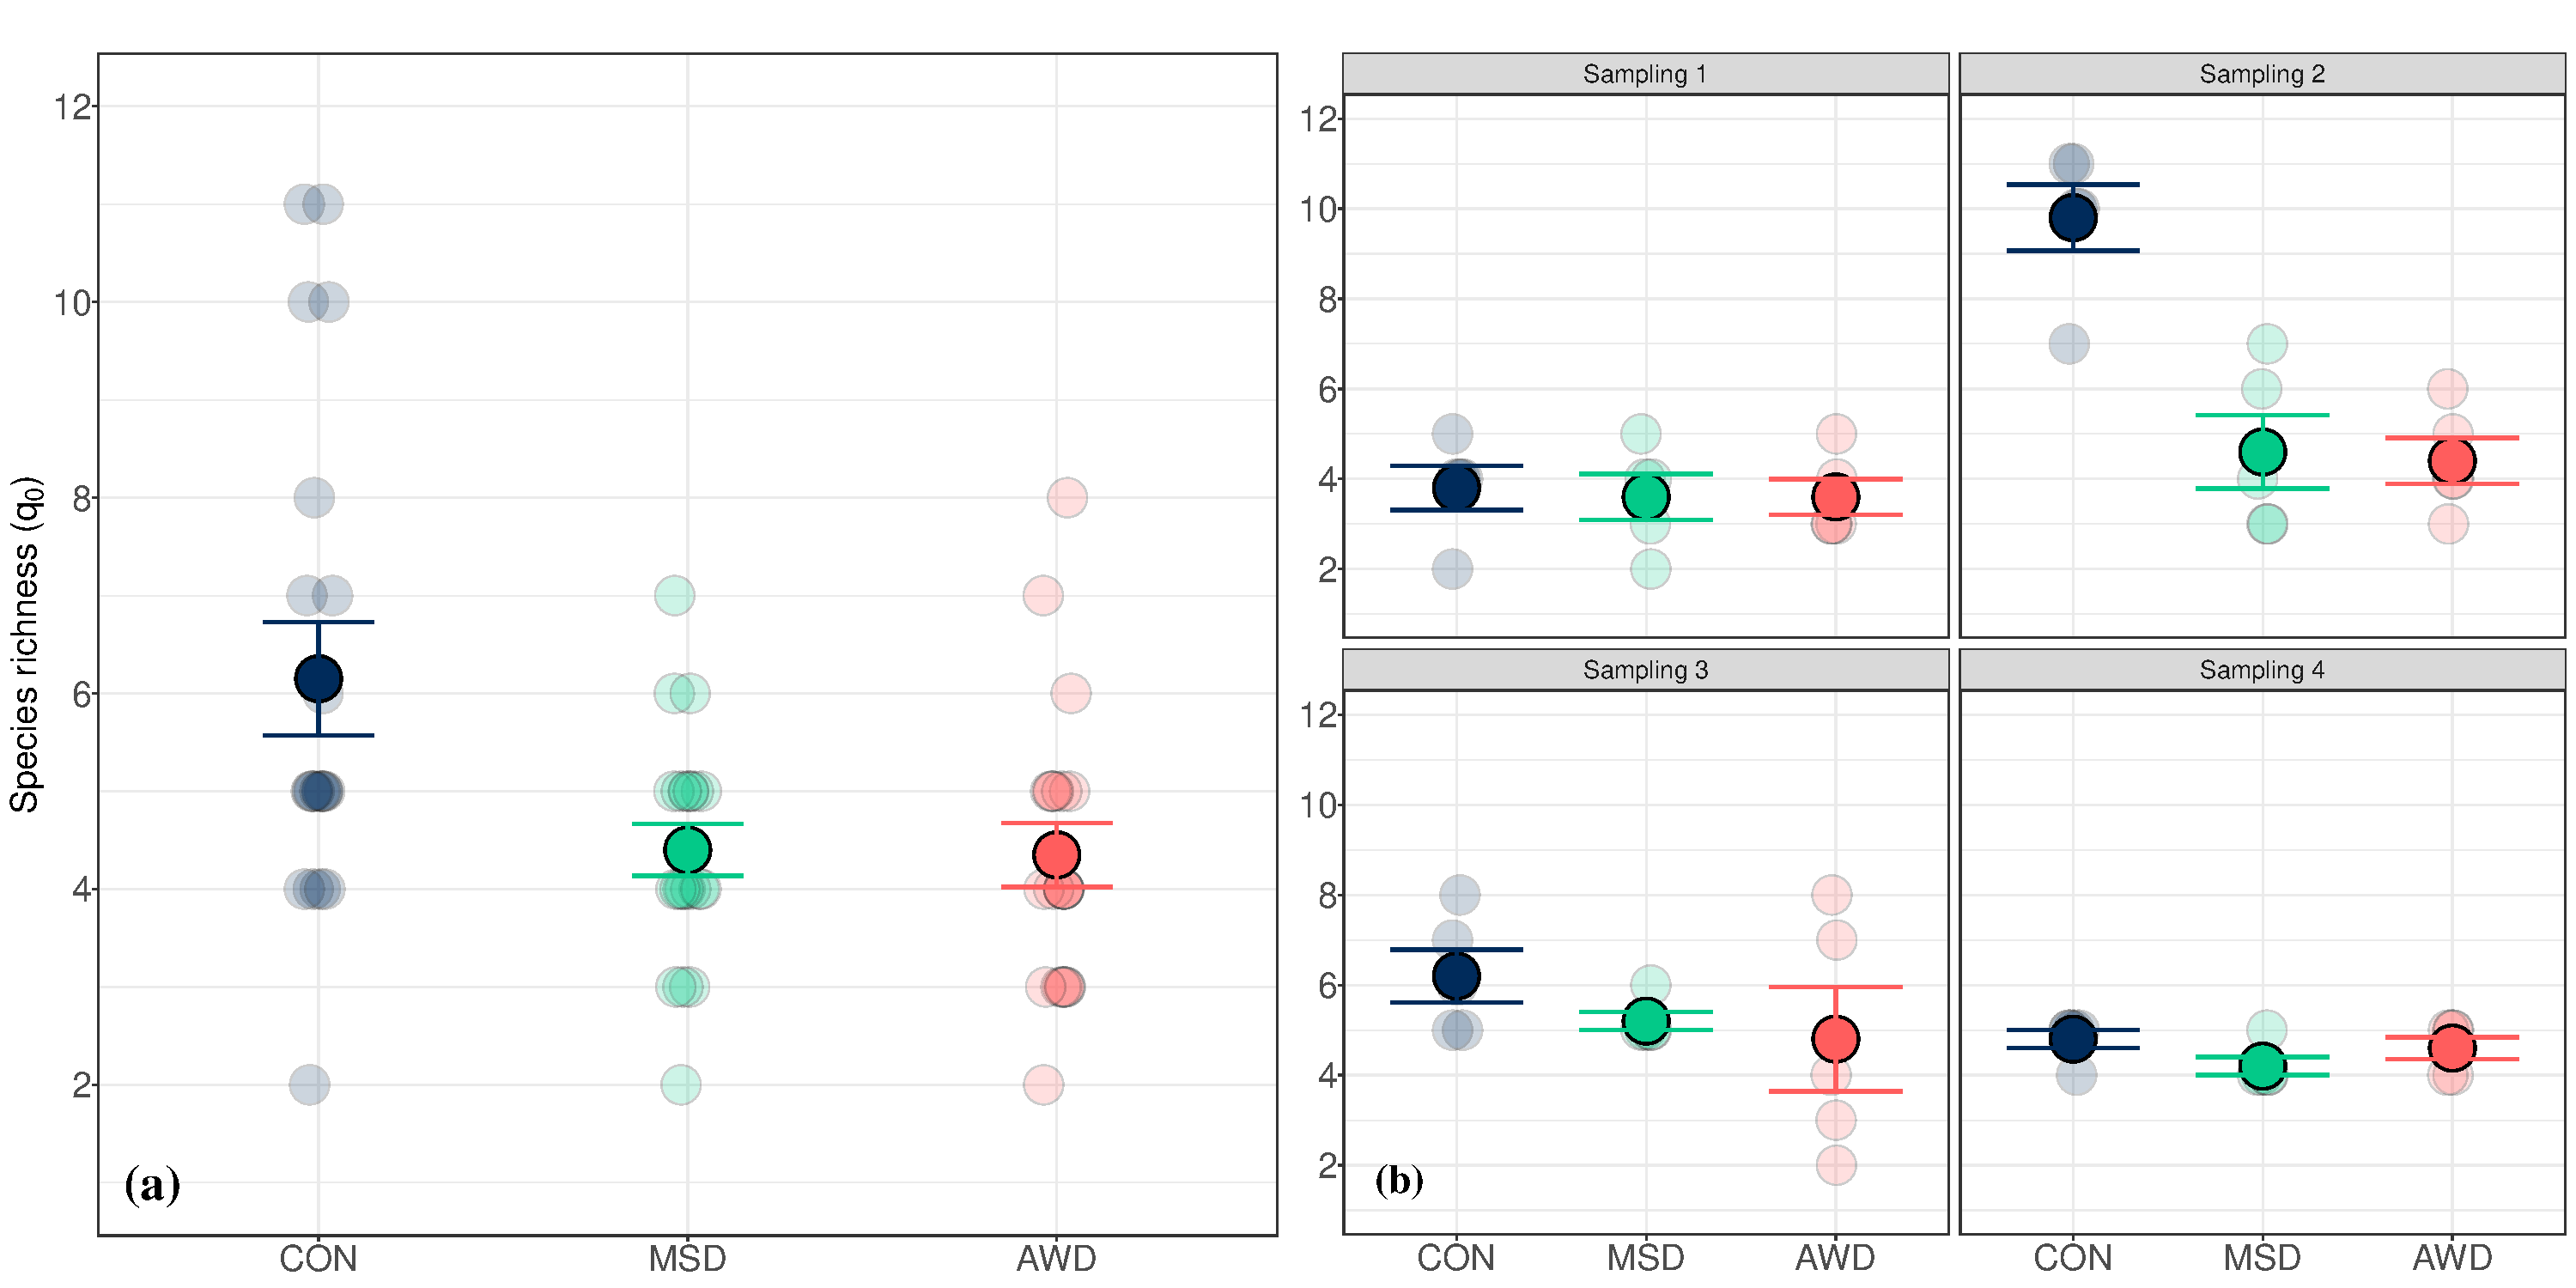
\includegraphics[scale=0.33, center]{Figures/Chapter_1/Arr.q0_ind.samp.pdf}
	\captionof{figure}[Species richness]{Macroinvertebrate species richness (number of identified species) for the three water-saving strategies. Semi-transparent points indicate plot means for each sampling date. Solid points and error bars indicate the overall means and standard errors, respectively. The left-hand panel \textbf{(a)} shows overall averaged results considering all four sampling dates across the rice growing season. The right-hand panels \textbf{(b)} show results for each sampling date separately. Abbreviations for assessed irrigation strategies stand for: CON = continuous flooding; MSD = mid-season drainage; and AWD = alternate wetting and drying.}   
	\label{Div_q0}
\end{figure}
%\vspace{0.5cm}

Shannon diversity varied significantly among different irrigation strategies ($\chi^2$=13.3, \textit{p}=0.001; Figure \ref{Div_q1}). Nevertheless, no significant effect was detected for AWD plots when comparing to continuous flooding strategy (\textit{t}=0.2, \textit{p}=0.973), while MSD resulted in lower diversity than both continuous flooding (\textit{t}=2.9, \textit{p}=0.017) and AWD (\textit{t}=-2.5, \textit{p}=0.040), contrary to the expected balancing effect. Significant effects were identified for sampling date ($\chi^2$=17.6, \textit{p}=$<$0.001), squared sampling date ($\chi^2$=17.4, \textit{p}=$<$0.001), soil pH ($\chi^2$=5.5, \textit{p}=0.018) and oxygen concentration ($\chi^2$=3.9, \textit{p}=0.047).

 \begin{figure} [ht]
\captionsetup{justification=justified}
	\centering 
	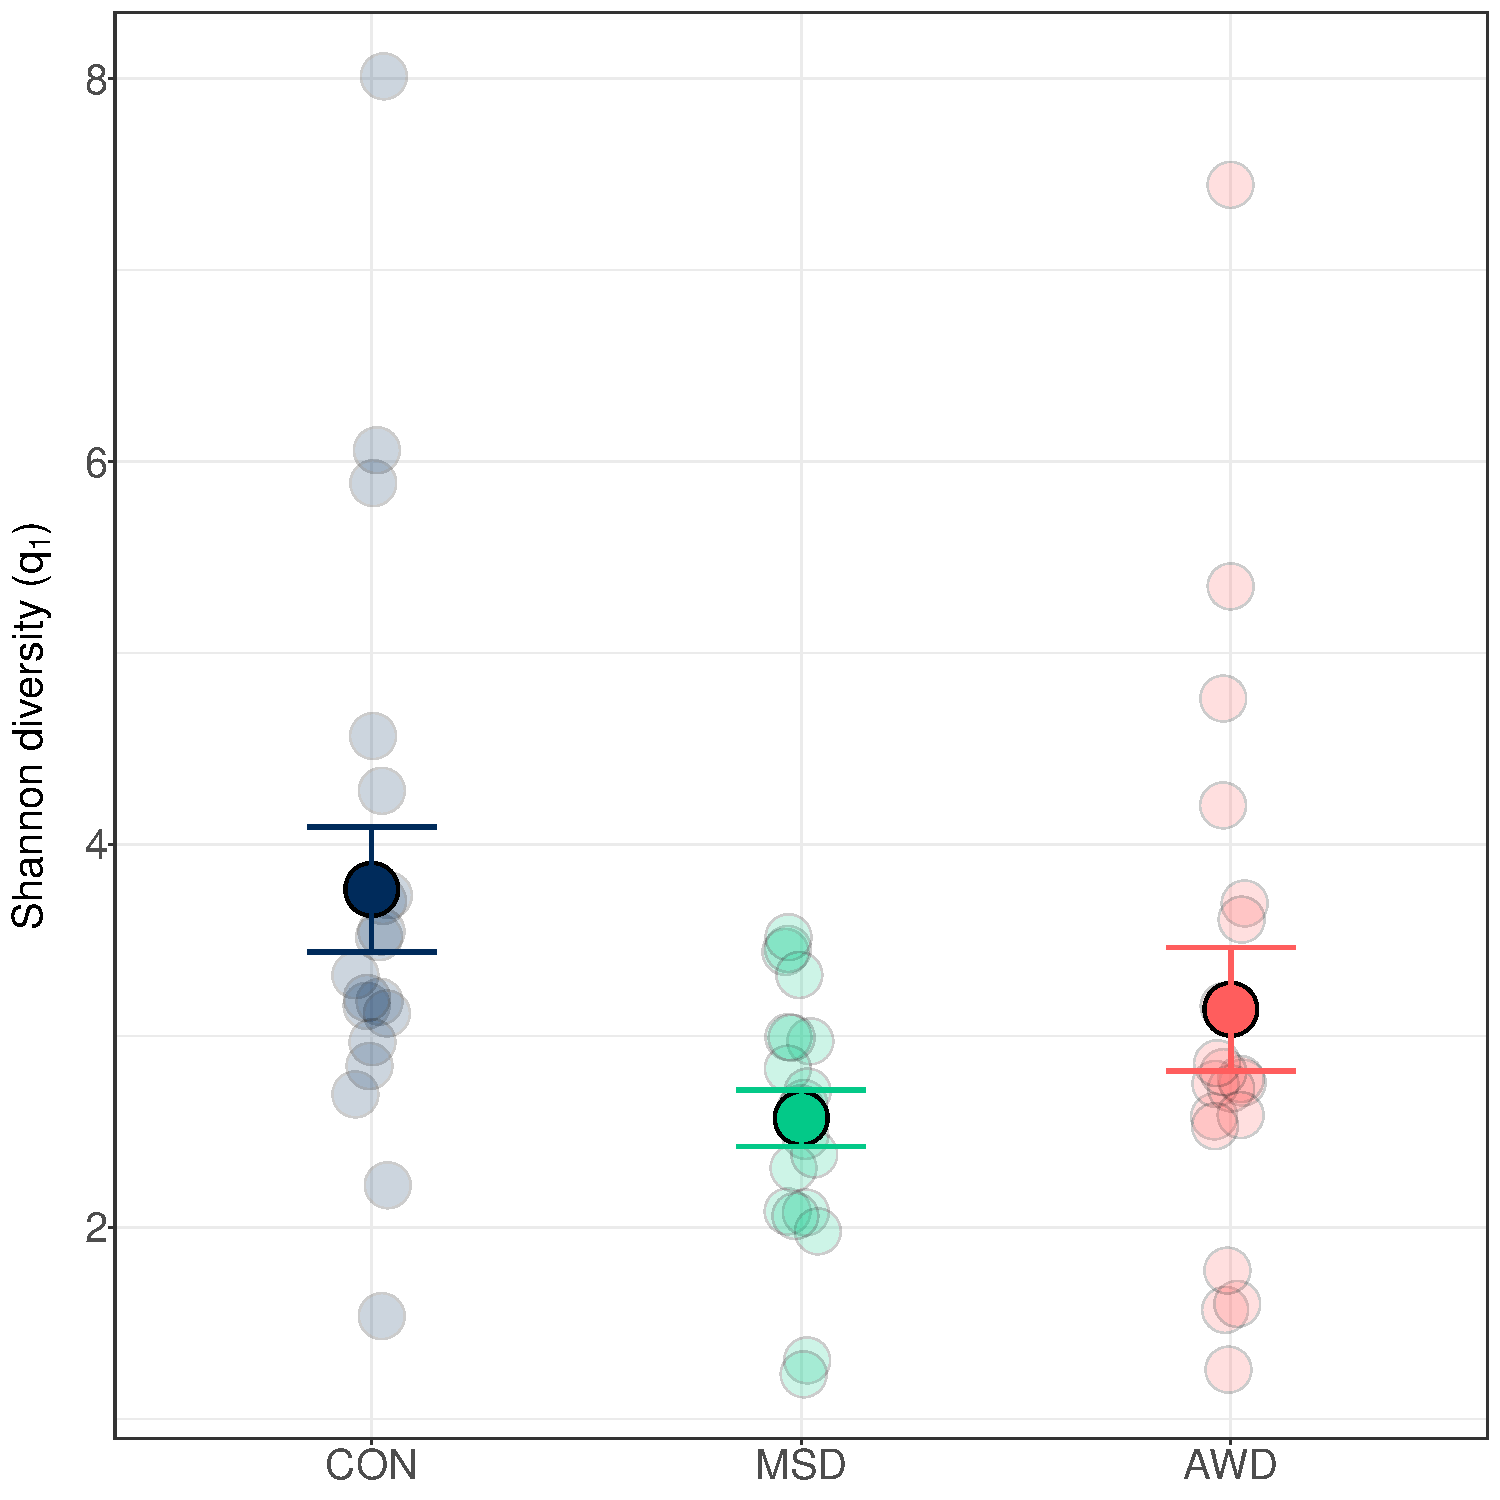
\includegraphics[scale=0.33, center]{Figures/Chapter_1/Shannon_indiv2.pdf}
	\captionof{figure}[Shannon diversity]{Macroinvertebrate Shannon diversity patterns for the three water-saving strategies. Semi-transparent points indicate plot means for each sampling date. Solid points and error bars indicate the overall means and standard errors, respectively. Abbreviations for assessed irrigation strategies stand for: CON = continuous flooding; MSD = mid-season drainage; and AWD = alternate wetting and drying.}   
	\label{Div_q1}
\end{figure}
%\vspace{0.5cm}

\subsection{Crop yield} 

Crop yields were influenced by water strategies (F=13.8, \textit{p}=$<$0.001). Implementing AWD as a high intensity and low water-use strategy, proved to reduce significantly final rice grain yield in comparison to both continuous flooding (\textit{t}=-4.4, \textit{p}=0.002, Figure \ref{Yields}) and MSD (\textit{t}=--4.7, \textit{p}=0.002) strategies. The mid-intensity MSD strategy, on the other hand, did not result in crop production declines against a continuous flooding strategy (\textit{t}=0.2, \textit{p}=0.968). Final mean yields were 8,213 ($\pm$176), 8,271 ($\pm$180) and 7,154 ($\pm$150) kg ha$^{-1}$, for plots under continuous flooding, MSD and AWD irrigation, respectively. A mean yield decrease of 12.9\% was observed for AWD when comparing to continuously flooded plots.

\begin{figure} [ht]
\captionsetup{justification=justified}
	\centering 
	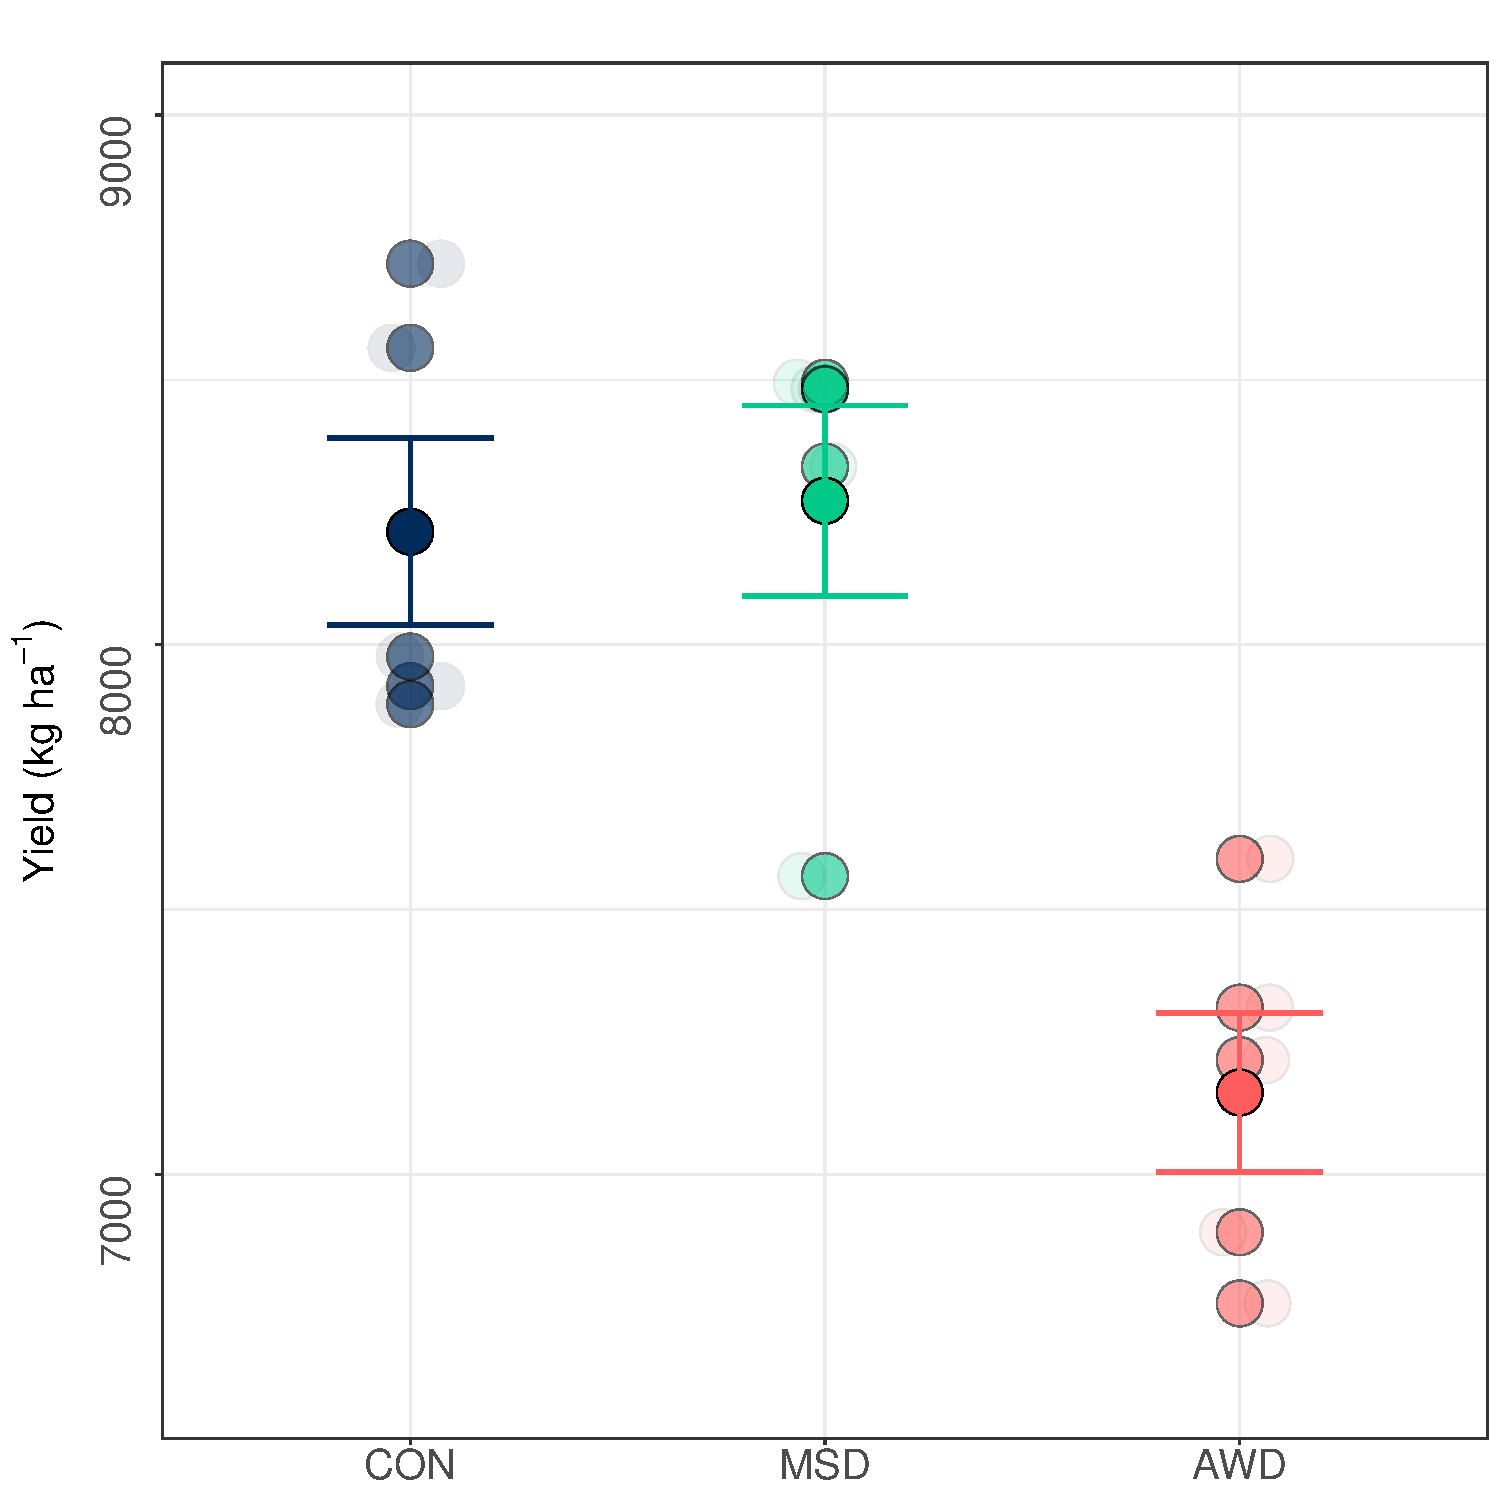
\includegraphics[scale=0.33, center]{Figures/Chapter_1/Prod_2022_plot2.pdf}
	\captionof{figure}[Yields]{Rice yields (kg h$^{-1}$) for all three water-saving strategies. Each bar shows the averaged yield for all plots according to each strategy, error bars indicate standard errors. Abbreviations for assessed irrigation strategies stand for: CON = continuous flooding; MSD = mid-season drainage; and AWD = alternate wetting and drying.}   
	\label{Yields}
\end{figure}
%\vspace{0.5cm}\\

\section{Discussion}
\label{sec:discussion}

Plenty of research effort has been focused on the development of water-saving irrigation strategies in rice paddy fields to adapt to more frequent severe droughts \citep{bouman2007, luo2019, shankar2021} and to mitigate climate change through a decline in CH$_{4}$ emission rates \citep{linquist2018}. Potential negative effects on biodiversity conservation of those species depending on rice water layers has, nevertheless, largely been overlooked. Through this study, the scope of agricultural management assessment is extended to include possible effects on these freshwater communities. \\

Regarding climate change mitigation, the assessed non-continuous flooding irrigation strategies resulted in positive effects, reducing CH$_{4}$ rates, as observed by several studies \citep{cai2003, li2006, lahue2016, lagomarsino2016, meijide2017}. Emission rates from AWD managed plots remained close to zero all across the flooding-drying cycle, pattern that has already been observed \citep{balaine2019}. This effect is attributed to aerobic oxidation by methanotrophs and reduced methanogenic activity \citep{kumar2019alternate}. Although a meta-analysis by \cite{jiang2019} found that non-continuous flooding practices reduced CH$_{4}$ emissions in average by 53\% compared to continuous flooding, these impacts are variable throughout the literature and high reductions as those observed in the present study (92.5\%) are in line with previous observations in temperate rice production regions. In Italy, \cite{peyron2016} eliminated completely CH$_{4}$ emissions through AWD, maintaining oxic conditions through most of the growing season. In California, AWD has been reported to decrease CH$_{4}$ emissions up to 87\% \citep{lahue2016} and 93\% \citep{linquist2015} in relation to continuous flooding, attributing such large effects to soils drying more in between flood events than in studies where no such large decreases were observed, and to drainage timing. Maximum emission decreases are achieved if drainage is implemented when \citep{fertitta-roberts2019}, or a few days before \citep{souza2021}, emission peaks are observed in continuously flooded fields. In regions in which CH$_{4}$ emissions peak early in the season (e.g. China), but keep fields flooded or drain them late in the growing season, there is a large mitigation potential to reduce CH$_{4}$ emissions \citep{qian2023}. Emissions from MSD plots increased similarly to those conventionally managed during the beginning of the season (mid- to late-June, Figure \ref{CH4_acc}), but collapsed to levels closer to AWD plots as soon as the drainage period was implemented. Right after these plots were re-flooded, emissions recovered steadily but did not return to continuous flooding levels. This two-peaked pattern in CH$_{4}$ emission fluxes has been observed frequently for MSD water management in rice paddy fields \citep{sass1992, yagi1997}. Emission rates and seasonal accumulated CH$_{4}$ emissions respond to the water-use gradient, with highest emissions in conventional plots and lowest in AWD plots \citep{islam2022, perry2022}. The MSD irrigation served, as expected, as a balancing strategy in between both gradient extremes. Results are in good agreement with those found in previous studies, which report reductions of up to 95.0\% for AWD \citep{martinez-eixarch2021} and 66.0\% for MSD \citep{balaine2019} in seasonal cumulative emissions, when compared to continuous flooding strategies.\\

The impact of water saving techniques on freshwater biodiversity in rice plots are evident when comparing abundance of aquatic organisms among differently irrigated plots. There is a marked negative effect on vertebrate and macroinvertebrate abundance when comparing AWD with both continuous flooding and MSD strategies. For most of the assessed groups of organisms, there is a decreasing trend in overall abundance, with more individuals sampled in continuously flooded plots, followed by MSD and, finally, AWD. Multiple short hydroperiods associated to AWD rice fields might avoid the completion of active aquatic phases for many invertebrates and amphibians \citep{lawler2001}. The strong abundance decline in aquatic macroinvertebrates present in AWD plots might be attributed to the fact that univoltine (one brood per season) predator insects are susceptible to drainage in intermittently irrigated rice fields, which might prove positive for multivoltine prey species, like mosquitoes \citep{mogi1993}. The impact of short hydroperiods is especially evident for amphibians, for which the absence of tadpoles in AWD managed plots indicated a collapse in \textit{Pelophylax perezi} recruitment. AWD managed plots act, therefore, as ecological traps for amphibians, which is the group of vertebrates most threatened by habitat transformation \citep{amphibians}. \cite{watanabe2013} reported negative effects of MSD irrigation on abundance in respect to continuous flooding irrigation. We observed similar or higher abundances for coleoptera, fish and amphibians in MSD plots compared to those continuously flooded, and lower abundances for decapoda, heteroptera and odonata, but not as low as those observed for AWD plots.\\ 

Effects on the diversity of aquatic macroinvertebrates (i.e., aquatic bugs, beetles and odonates) were more subtle than those observed for their abundance. Even though overall species richness did not seem affected considering all four samplings across the entire season (Figure \ref{Div_q0}a), there was a clear effect on the second sampling (Figure \ref{Div_q0}b), which was carried out several days after both non-continuously flooded strategies went through a drained period and were re-flooded. Comparing the first sampling results, in which all plots had been equally flooded and species richness was equivalent, to the second one, there is a clear increase in species present in continuous flooded plots in contrast to stagnated MSD and AWD levels. Even though community dynamics in temporary wetlands are driven by multiple factors, such as flooding timings and functional traits of aquatic species \citep{schneider1996, boix2016}, removing water layers might have drastically affected the number of present species in non-continuous flooding strategies, as species richness generally increases with longer hydroperiods \citep{batzer1996}. \cite{perez2023enhanced} observed that species richness peaks during the middle of rice growing season. Therefore, drainage in MSD and AWD managed plots previous to this mid-season peak may explain the species richness decline at this moment and all through the remaining growing season. The effects of low conductivity and high oxygen concentration as drivers of higher species richness for aquatic macroinvertebrate communities have been previously identified \citep{graca2004, waterkeyn2008, boix2010, brucetbalmana2012, croijmans2021, mazzoni2023}. \added[id=SE]{Decreases in oxygen levels might result from stagnant water during drain cycles, in contrast to constant flow in continuously flooded plots}. Less evident effects were recorded when looking at Shannon diversity, where high variability was observed for continuous flooding and AWD strategies and, therefore, no significant differences were identified between them. MSD resulted in less diversity, yet this could be attributed to regular changes in community dynamics. Lower diversity levels in MSD plots than in AWD ones might contradict the principles behind the intermediate disturbance hypothesis, in which increasing disturbance drives towards higher diversity up to a certain threshold \citep{dial1998}, but further analysis into community dynamics would be required to assess if higher disturbance levels induced by AWD management drive towards higher coexistence between dominant and subordinate species. Studies resulting in different trends, such as higher diversity in MSD managed plots than in continuously flooded ones \citep{watanabe2013}, suggest that irrigation effects on biodiversity might be species- and/or site-specific and that more research, and at longer spatial and temporal scales, should be done to identify the main drivers behind such dynamics.\\

Evidence suggests that the outcomes of the alternative irrigation strategies go beyond the purely environmental effects, affecting as well crop yields. A mean production loss of 5.4\%, and as high as 22.6\%, depending on the intensity of implementation, has been observed for AWD irrigation, as alternative to continuous flooding \citep{carrijo2017}. \added[id=SE]{Even though high seasonal variation lead \cite{martinez-eixarch2021} to conclude non-significant differences in grain yield when comparing AWD and continuous flooding irrigation on the same study site, they observed an average 12\% decrease for AWD plots (19\% and 6\% grain yield decreases versus continuous flooding for seasons 2016 and 2017, respectively).}\added[id=SE]{ That previous study identified high annual variability and dependence on agronomic parameters (i.e., rice cultivar) for grain yields under AWD irrigation. Despite this, the overall yield decline is aligned with the 12.9\% yield reduction observed in the present study.} Although final yield decreased, the decline is lower than experiments that implemented more severe AWD, with longer drying periods \citep{tabbal2002}. Nevertheless, higher water use efficiency (i.e., produced grain per water input) has been identified as a potential benefit of this practice \citep{wassmann2009regional}. Even though AWD treatment was performed under Safe-AWD protocol, soils high in clay are prone to result in yield losses even under such practices, mainly because these may still get too dry to avoid plant water stress \citep{carrijo2017}. Besides water stress, AWD might reduce yields due to potential lower N uptake, as a result of N losses by nitrification and denitrification \citep{pandey2014}. Regarding MSD, drops in rice production levels were not only minimized, as expected initially with the implementation of this mid-intensity strategy, but were kept intact when compared to continuously flooded plots productivity. Unaltered crop yields under MSD in regards to continuous flooding have previously been observed \citep{perry2022}. While such positive results might point towards the implementation of mid-season drainage as a an effective water saving strategy without negative effects on yield, attention should be put on potential long-term sustainability, as it might decrease soil fertility \citep{livsey2019} and result in diminished provision of ecosystem services such as biological pest control, organic matter decomposition and nutrient cycling \citep{nicholls1998, prather2013}.  \\

\section{Conclusions}
\label{sec:conc}

Decisions regarding agricultural management should be assessed considering the multiplicity of its impacts. In this study, practices aimed at achieving climate change mitigation and adaptation to severe droughts, while avoiding production declines, are shown to have negative impacts on biodiversity conservation. Such contradicting outputs can be offset by testing alternative practices that do consider multiple goals. While management focused on fewer objectives might achieve higher outcomes regarding them, alternative multi-objective strategies allow production within a positive range of results for all considered goals and avoids overseeing potential negative effects due to lack of consideration. Such more holistic approaches are to be promoted, as they lead to more sustainable production in the long term. \\

Rice production has been undergoing a process of innovative transformation from traditional practices, as it faces challenges regarding climate change and increasing food demand. While intermittent irrigation addresses CH$_{4}$ emissions and water requirements, it might cause detrimental effects on biodiversity conservation goals if widely, and indiscriminately, implemented. \added[id=SE]{In our particular case study, AWD resulted in strong abundance and grain yield declines, highlighting the need to assess it locally before its implementation within similar systems. }\added[id=SE]{Effects on biodiversity, even if not observed throughout the entire rice season, might occur during critical stages in which biodiversity peaks would, otherwise, be expected.} Alternative, medium-intensity, irrigation practices such as mid-season drainage might hinder\added[id=SE]{, at least partially,} these negative effects and serve as more conciliatory strategies.\replaced[id=SE]{ In this study, MSD}{This practice} accomplished to reduce CH$_{4}$ emission rates in regards to continuous flooding, while also avoiding production loss and drastic abundance decrease in aquatic communities when compared to alternate wetting and drying management. \replaced[id=SE]{However, a single drain had a negative effect on Shannon diversity, whereas this was not the case for AWD managed plots, when compared to continuous flooding. }{However, Shannon diversity was negatively affected by a single drain when compared to other practices.}Therefore, deeper analyses of potential effects of \replaced[id=SE]{performing a single mid-season drain}{ this strategy} on the diversity and spatiotemporal dynamics of aquatic organisms should be done to assess its wider implementation.\\

This study encourages further discussion on the optimum scope of agricultural management assessments given current and projected scenarios. Nevertheless, recognizing time and spatial scale limitations, longer term experiments under a wider range of conditions are required to identify specific management practices fitting\added[id=SE]{ different} scenarios\deleted[id=SE]{ that differ from that framing this study}. Long term effects should be analyzed to assess alternative, and potentially conciliatory, practices. Only through more integrative perspectives, innovations needed to tackle climate, biodiversity and production challenges can be developed without compromising sustainability.\\

\section*{ACKNOWLEDGEMENTS}
\label{sec:ackn}

This study was funded by the Spanish Ministry of Economy, Trade and Enterprise (MINECO) through the Grant PID2020-118650RR-C31 (funded by MCIN/ AEI/ 10.13039/ 501100011033). The Government of Catalonia funded the predoctoral fellwoship of S.E.-P. through the projects AgriCarboniCat and AgriRegenCat. N.P.-M. is supported by a Spanish ‘Ramón y Cajal’ fellowship (RYC-2021-033599-I). We thank Carles Alcaraz for his guidance in regards to data analysis. We also thank Andrea Bertomeu, Vicent Cebolla, Joan Didac Bertomeu and Juan Blas Fernández-Araujo for their field support and implementation of water strategies. The support of the CERCA Programme, Generalitat de Catalunya, is also acknowledged.

\subsection*{Competing interests statement}
\label{sec:interests}

The authors declare that they have no known competing financial
interests or personal relationships that could have appeared to influence the work reported in this paper.

%\pagebreak - SEBA: made note
 
% \bibliography{Paper_1_bib}  - SEBA: made note

\pagebreak

%\appendix
%\section*{Appendices}
%\label{sec:ann}
%
%\setcounter{figure}{0}
%\renewcommand{\thefigure}{A.\arabic{figure}}

\section{Appendix to Chapter 1}
\addcontentsline{toc}{chapter}{Appendix to Chapter 1}
\renewcommand{\thefigure}{A.\arabic{figure}}
\setcounter{figure}{0}
\renewcommand{\thetable}{A.\arabic{table}}
\setcounter{table}{0}

% Layout:

\begin{figure*}[htbp]
\captionsetup{justification=justified}
	\centering 
	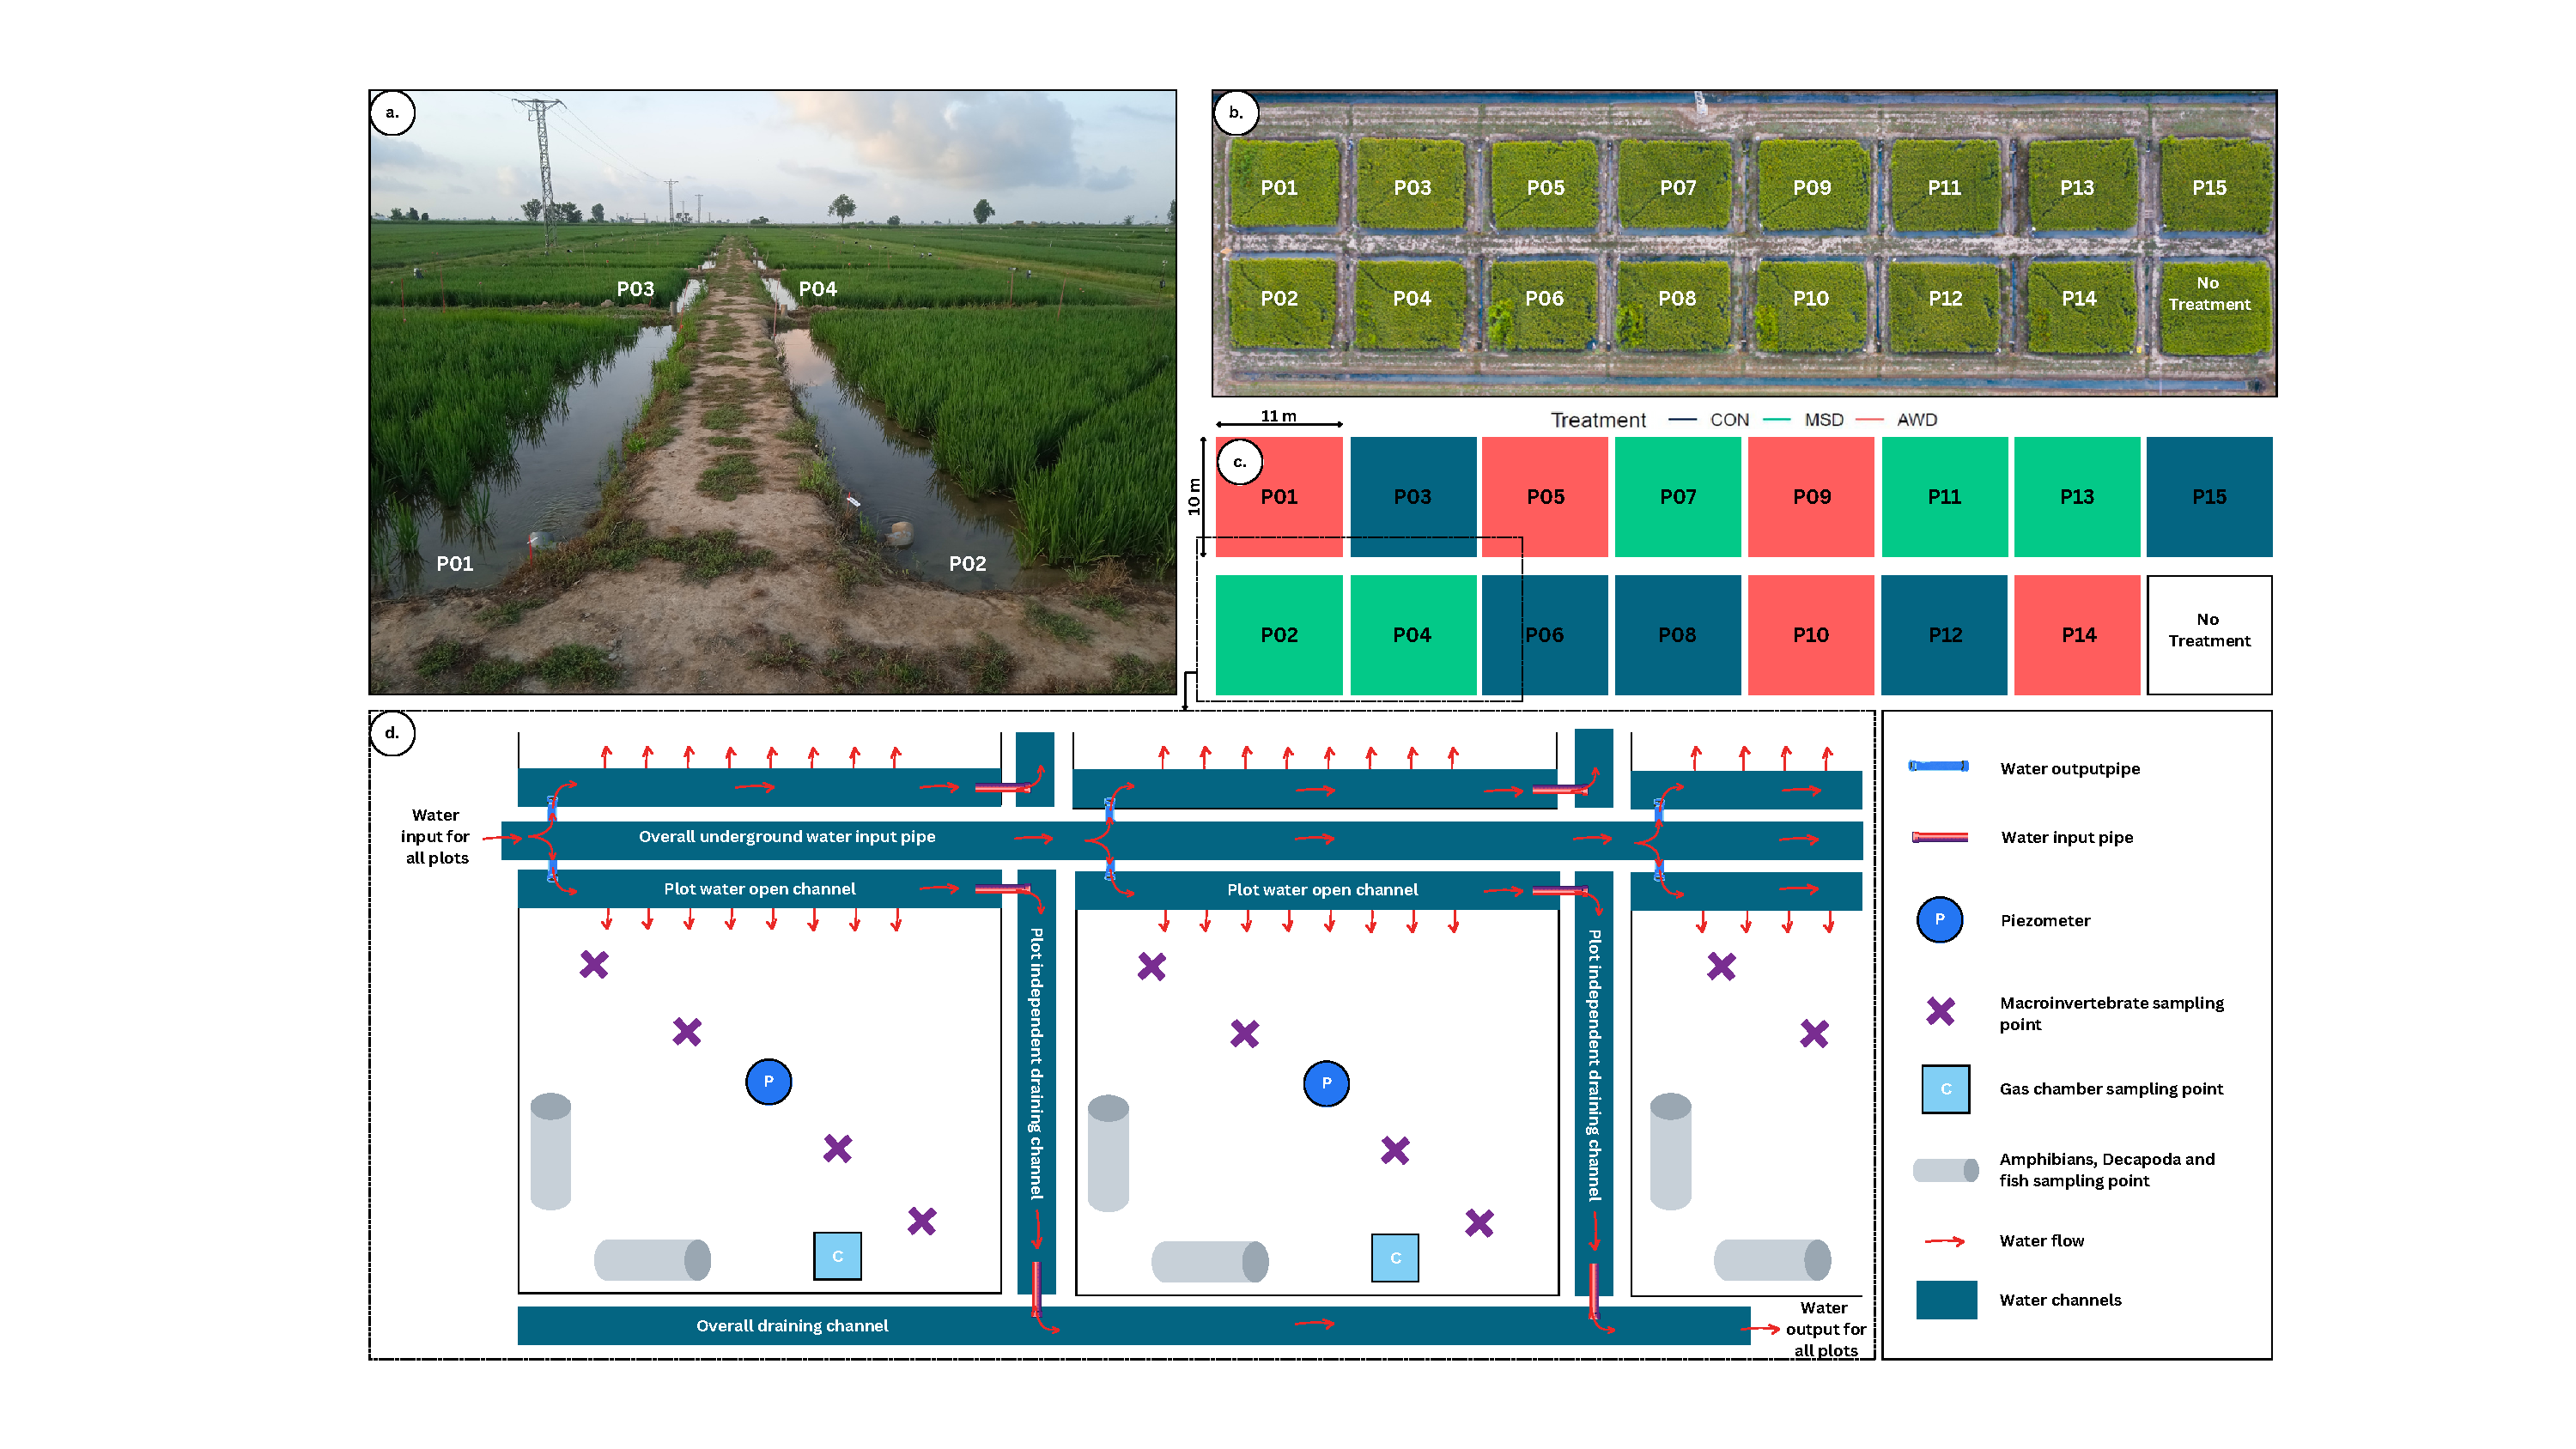
\includegraphics[scale=0.4, center]{Figures/Chapter_1/CERESTRES_layout.pdf}
	\captionof{figure}[Treats]{Experimental layout. \textbf{a.} Ground level view of experimental plots. \textbf{b.} Aerial view. \textbf{c.} Spatial distribution of water treatments. \textbf{d.} Water channelization system and sampling points within plots. Water management was independent for each plot as inputs and outputs could be opened and closed according to the assigned water strategy and thanks to each plot having its own independent draining channel on one of its sides. Piezometers, used to track water level, were installed only in MSD and AWD plots. All samplings (i.e, chambers for greenhouse gases emissions; cylindrical static nets for amphbians, decapoda and fish; and dip net sampling for macroinvertebrates) were repeated in the same location within plots for each sampling date. Abbreviations for assessed irrigation strategies stand for: CON = continuous flooding; MSD = mid-season drainage; and AWD = alternate wetting and drying.}   
	\label{Exp.lay}
\end{figure*}
%\vspace{0.5cm}\\

% CH4 alt. models example:

\begin{figure*}[htbp]
\captionsetup{justification=justified}
	\centering 
	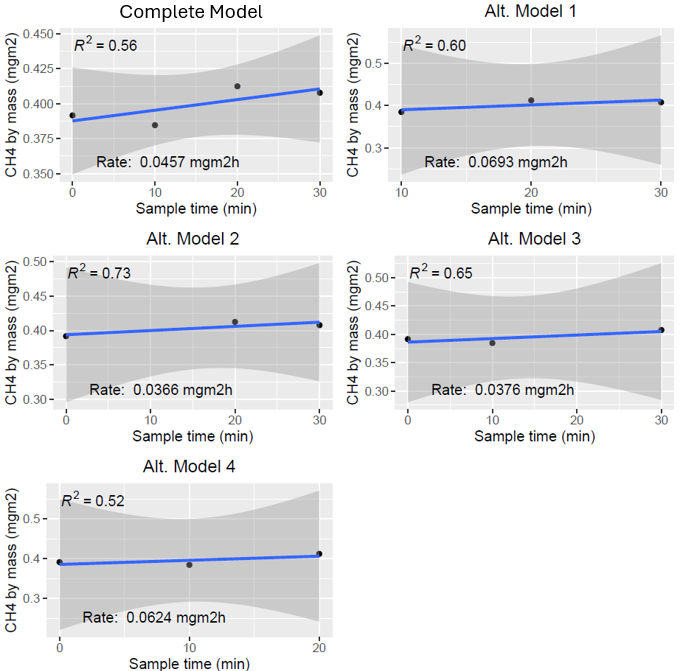
\includegraphics[scale=0.8]{Figures/Chapter_1/mod_exp.png}
	\captionof{figure}[varsTreat]{Example of alternative CH$_{4}$ flux models. The first panel (top-left) shows the complete model, with all four concentration measurements, for one sampling event. This model achieved R$^{2}$ = 0.56. The following four panels show alternative models, each dropping one of the four measurements (e.g. Alt. Model 3 drops the min=20 measurement and keeps measurements min 0; 10; and 30). For this sampling event the alternative model 2 (dropping measurement min=10) is the only one achieving R$^{2}$ $>$ 0.7, thus being considered as corrected CH$_{4}$ flux.)}  
	%\refstepcounter{SIfig}
 \label{mod_exp}
\end{figure*}

% Correlation:

\begin{figure*}[htbp]
\captionsetup{justification=justified}
	\centering 
	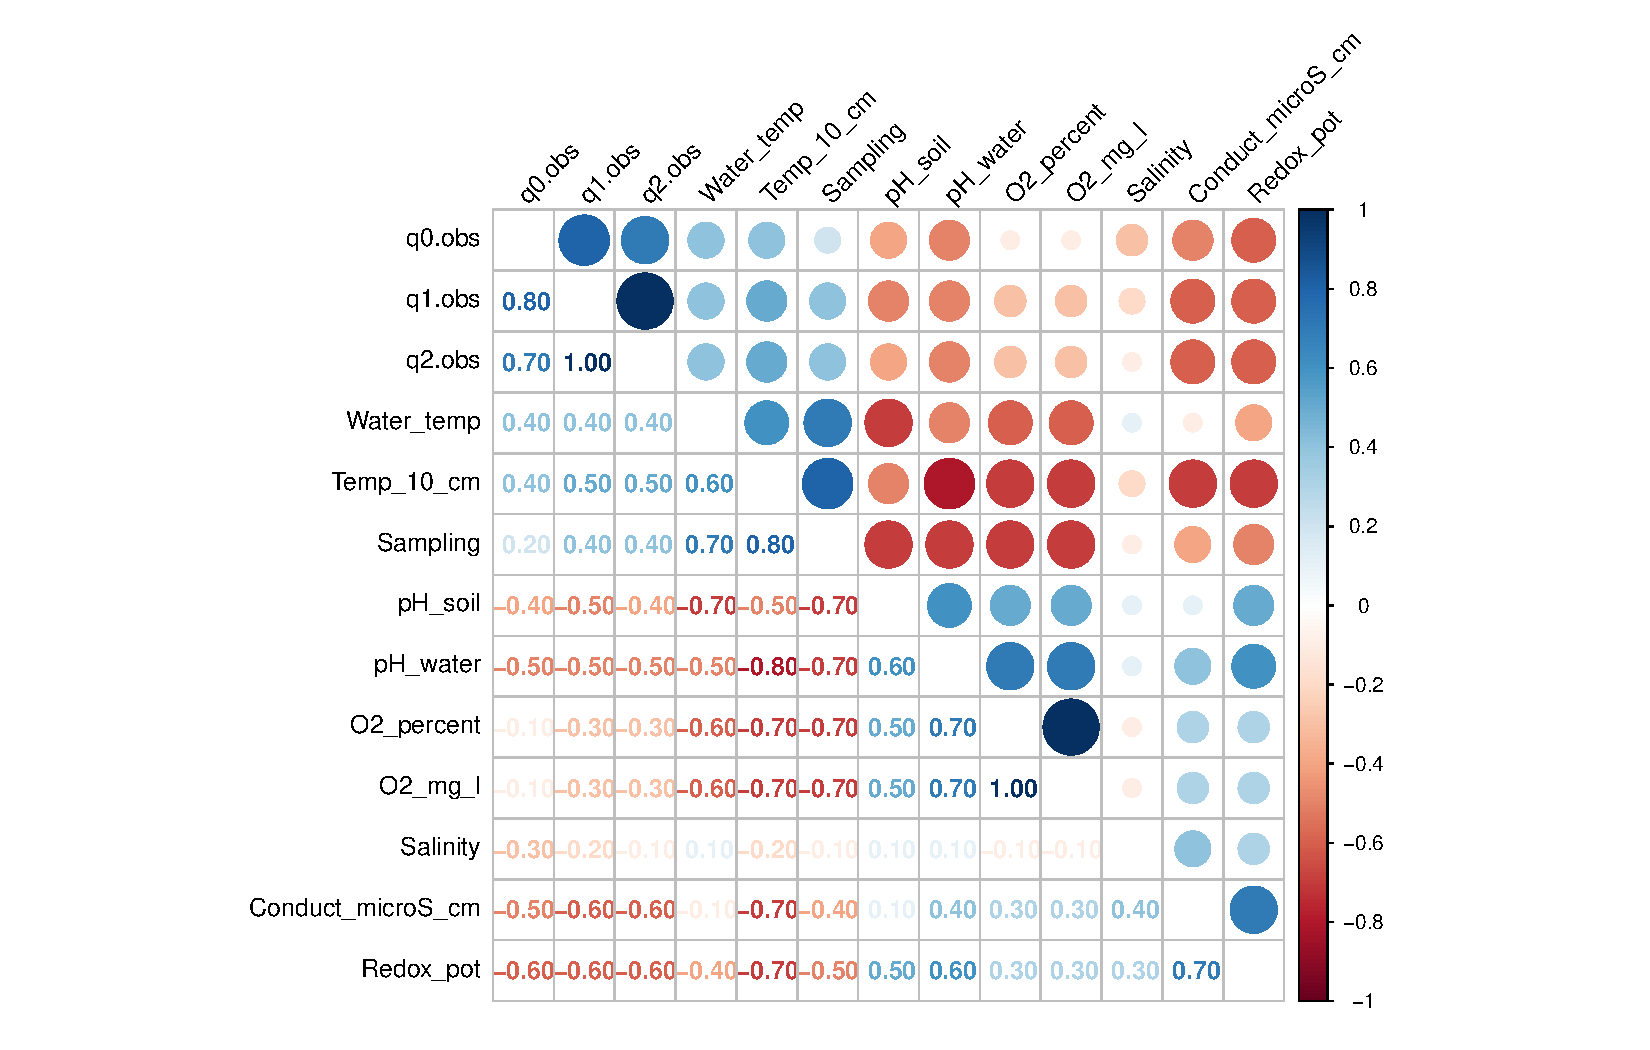
\includegraphics[scale=0.4, center]{Figures/Chapter_1/Corr_plot_nooutliers.pdf}
	\captionof{figure}[varsTreat]{Spearman's rank correlation coefficient in between soil and water physicochemical covariates, and biodiversity components (q0.obs = Species richness, q1.obs = Shannon diversity). Red circles represent negative correlation and blue circle positive correlation among variables. The size of circles is positively related to correlation among variables.}  
	%\refstepcounter{SIfig}
 \label{Corr_plot}
\end{figure*}

% Dendrogram:

\begin{figure*}[htbp]
\captionsetup{justification=justified}
	\centering 
	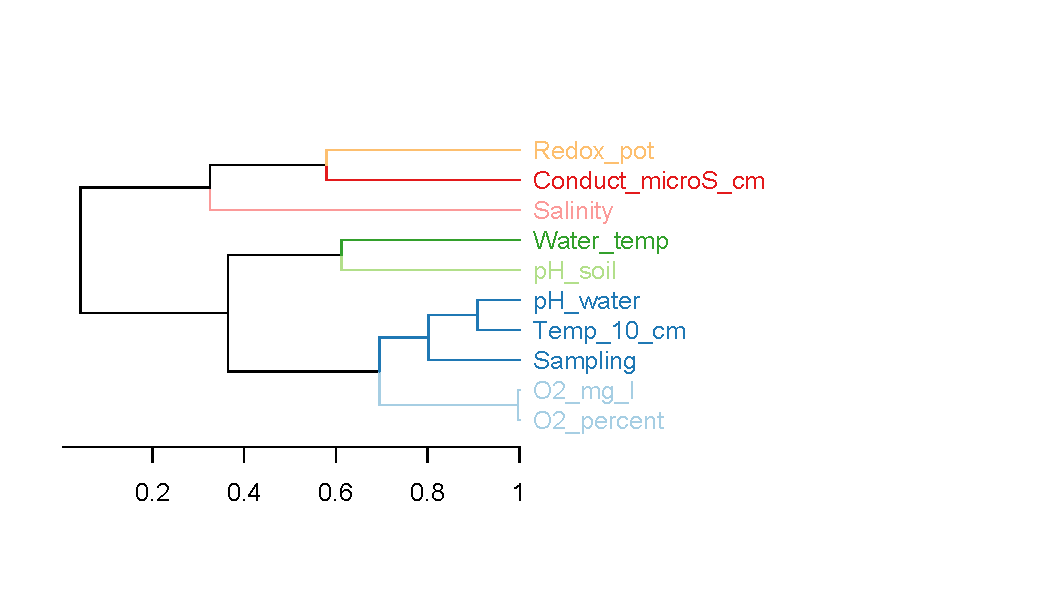
\includegraphics[scale=0.6, center]{Figures/Chapter_1/Cluster_variables_pearson_5_nooutliers2.pdf}
	\captionof{figure}[varsTreat]{Dendrogram based on the Pearson correlation coefficient for soil and water physicochemical covariates.}  
	%\refstepcounter{SIfig}
 \label{Dendro}
\end{figure*}

% Physchem variables vs Treat boxplots:

\begin{figure*}[htbp]
\captionsetup{justification=justified}
	\centering 
	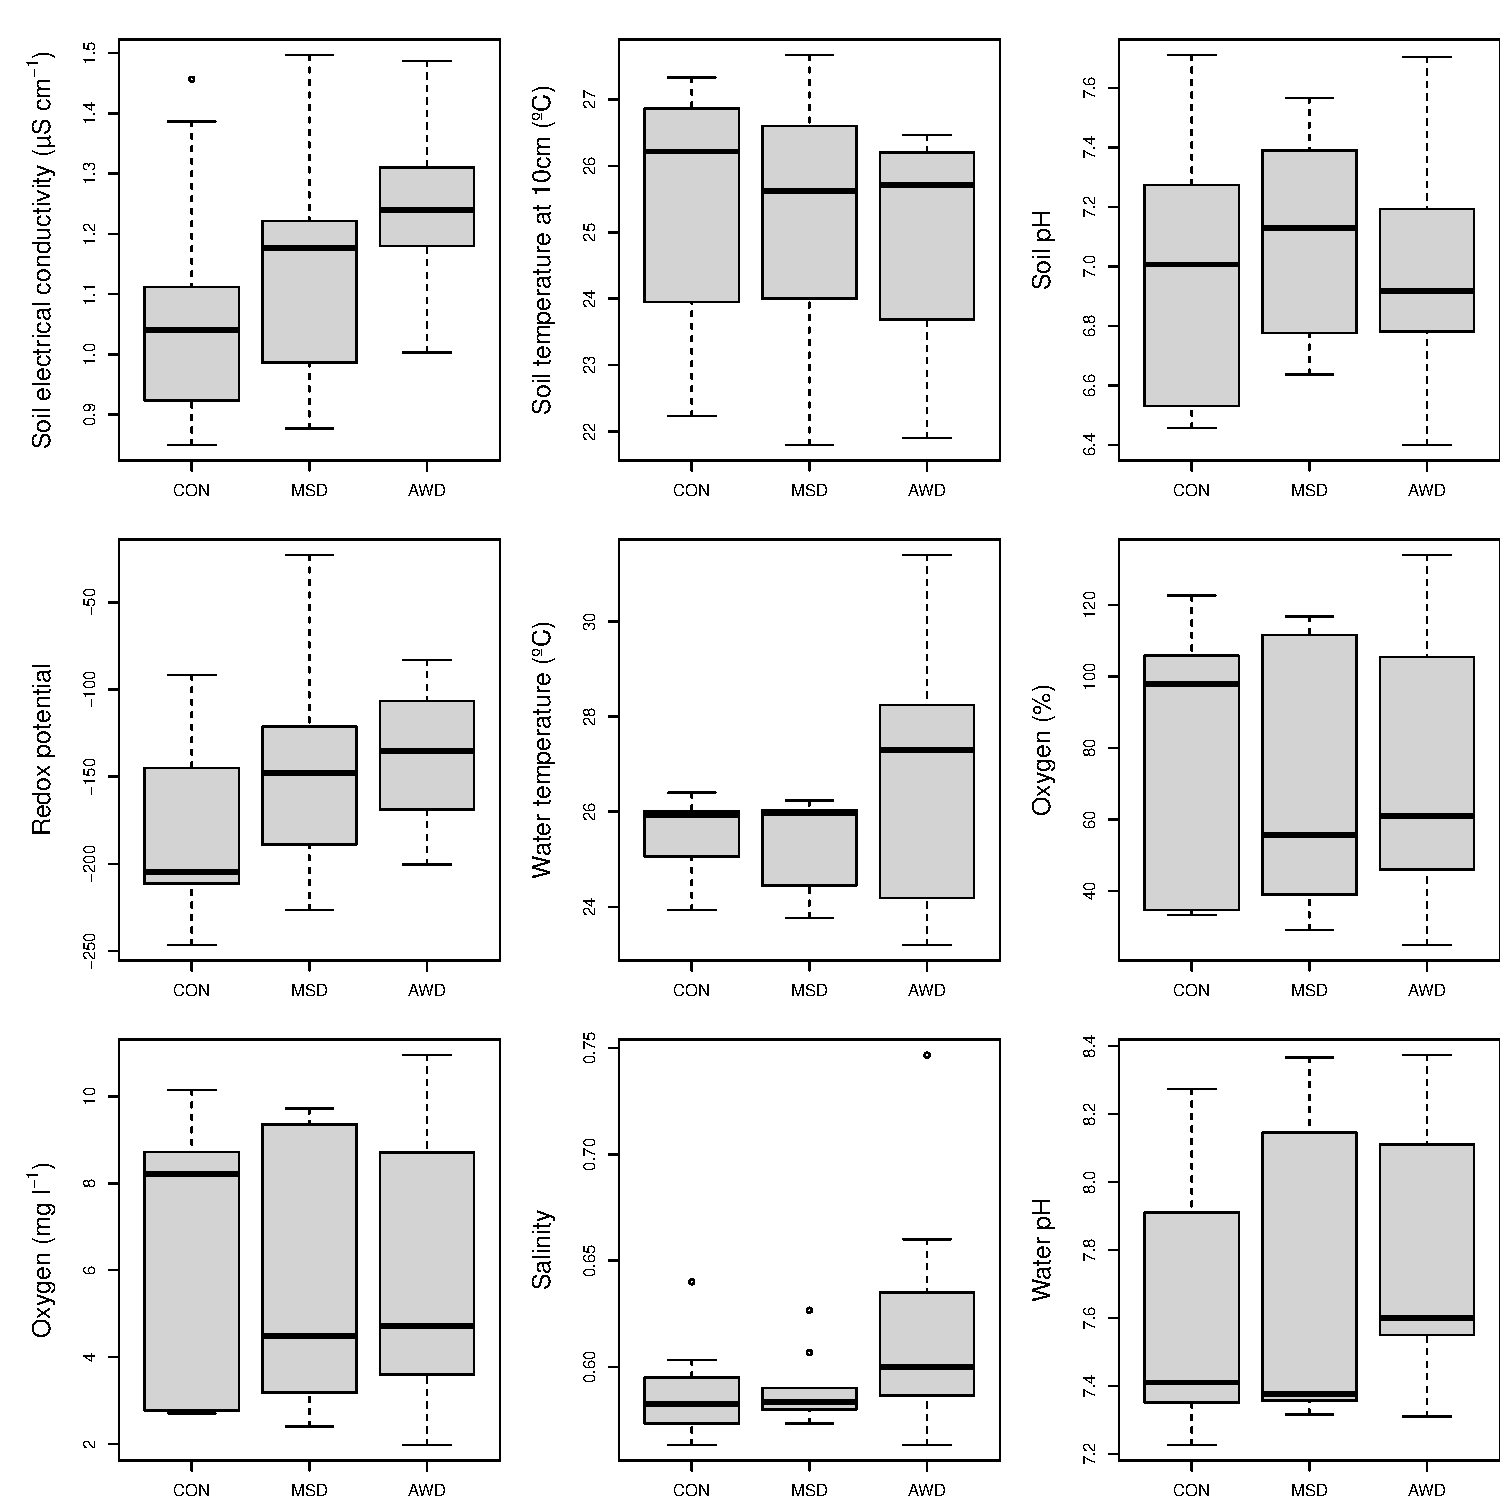
\includegraphics[scale=0.6, center]{Figures/Chapter_1/Ind_vars_Treat_inter.pdf}
	\captionof{figure}[varsTreat]{Soil and water physicochemical parameters for each water-saving irrigation strategy. Abbreviations for assessed irrigation strategies stand for: CON = continuous flooding; MSD = mid-season drainage; and AWD = alternate wetting and drying.}  
	%\refstepcounter{SIfig}
 \label{vars_Treat}
\end{figure*} 

\setcounter{table}{0}
\renewcommand{\thetable}{A.\arabic{table}} % Applies "A.1", "A.2", etc. format to appendix tables

\begin{table*} [htbp]
    \centering
    \scriptsize  
    \begin{tabular}{l | l | c c c c | c c c c | c c c c}
    \cline{1-14}
\multirow{2}{2.3cm}{Order} & \multirow{2}{3cm}{Maximum taxonomy} & \multicolumn{4}{c}{Continuous Flooding}  & \multicolumn{4}{c}{MSD} &  \multicolumn{4}{c}{AWD}  \\
    \cline{3-14}
& & S1 & S2 & S3 & S4 & S1 & S2 & S3 & S4 & S1 & S2 & S3 & S4\\
    \cline{1-14}
\multirow{6}{2.3cm}{Coleoptera}  & \textit{Enochrus  sp.} & 0 & 0 & 1 & 0 & 0 & 0 & 1 & 0 & 0 & 0 & 7 & 0\\
& Fam. Hydrophilidae & 0 & 0 & 0 & 0 & 0 & 0 & 0 & 1 & 0 & 0 & 0 & 2\\
& \textit{Helochares sp.} & 1 & 14 & 0 & 0 & 1 & 3 & 2 & 0 & 0 & 3 & 4 & 0\\
& \textit{Hydaticus  sp.} & 0 & 1 & 0 & 0 & 0 & 2 & 1 & 0 & 0 & 2 & 0 & 0\\
& \textit{Hydroglyphus sp.} & 148 & 27 & 1 & 0 & 220 & 0 & 0 & 0 & 155 & 14 & 5 & 0\\
& \textit{Rhantus suturalis} & 0 & 0 & 0 & 0 & 1 & 0 & 0 & 0 & 3 & 0 & 0 & 0\\
    \cline{1-14}
\multirow{5}{2.3cm}{Hemiptera} & \textit{Anisops sardeus} & 0 & 25 & 16 & 32 & 0 & 2 & 36 & 10 & 0 & 1 & 3 & 15\\
& \textit{Gerris sp.} & 0 & 33 & 6 & 0 & 0 & 3 & 1 & 0 & 0 & 1 & 0 & 0\\
& \textit{Mesovelia vittigera} & 0 & 17 & 2 & 2 & 0 & 7 & 2 & 4 & 0 & 0 & 1 & 2\\
& \textit{Microvelia pygmaea} & 0 & 163 & 72 & 74 & 0 & 57 & 65 & 82 & 0 & 20 & 27 & 147\\
& \textit{Sigara nigrolineata} & 17 & 25 & 9 & 1 & 16 & 1 & 25 & 0 & 5 & 7 & 0 & 6\\
    \cline{1-14}
\multirow{7}{2.3cm}{Odonata} & \textit{Coenagrion sp}. & 0 & 6 & 0 & 1 & 0 & 4 & 0 & 0 & 0 & 0 & 0 & 0\\
& Fam. Coenagrionidae & 23 & 0 & 0 & 0 & 13 & 0 & 0 & 0 & 11 & 0 & 0 & 0\\
& Fam. Libellulidae & 41 & 0 & 0 & 0 & 15 & 0 & 0 & 0 & 13 & 0 & 0 & 0\\
& \textit{Ischnura elegans} & 0 & 155 & 178 & 33 & 0 & 8 & 145 & 25 & 0 & 27 & 7 & 36\\
& \textit{Ischnura graellsii} & 0 & 9 & 37 & 13 & 0 & 0 & 0 & 6 & 0 & 0 & 0 & 24\\
& \textit{Sympetrum fonscolombii} & 0 & 14 & 4 & 0 & 0 & 0 & 0 & 0 & 0 & 0 & 3 & 0\\
& \textit{Sympetrum lefebvrii} & 0 & 2 & 0 & 0 & 0 & 0 & 0 & 0 & 0 & 0 & 0 & 0\\

    \cline{1-14}
    \end{tabular}
    \caption{Macroinvertebrate abundance in number of sampled individuals. Organisms are presented according to the maximum taxonomical resolution achieved during the identification process. Fam. and sp. indicate individuals that could be identified up to Family and Genus levels, respectively. S1 to S4 indicate each of the four macroinvertebrate samplings. Abbreviations for assessed irrigation strategies stand for: MSD = mid-season drainage; and AWD = alternate wetting and drying.}
    \label{AbuColOdoHet}
\end{table*}


\begin{table} [htbp]
    \centering
    \scriptsize  
    \begin{tabular}{l | l | c c c c c c c c }
\cline{1-10}
\multirow{2}{2.3cm}{Order} & \multirow{2}{3cm}{Species} & \multicolumn{8}{c}{Continuous Flooding} \\
    \cline{3-10}
& & S1 & S2 & S3 & S4 & S5 & S6 & S7 & S8 \\
    \cline{1-10}
Anura & \textit{Pelophylax perezi} & 0 & 89 & 25 & 1 & 0 & 0 & 0 & 0\\
    \cline{1-10}
Decapoda & \textit{Procambarus clarkii} & 3 & 28 & 27 & 112 & 188 & 248 & 152 & 118\\
    \cline{1-10}
\multirow{3}{2.3cm}{Cypriniformes} & \textit{Carassius carassius} & 3 & 0 & 1 & 0 & 0 & 0 & 0 & 0\\
  & \textit{Misgurnus anguillicaudatus} & 0 & 0 & 1 & 2 & 0 & 1 & 2 & 0\\
& \textit{Pseudorasbora parva} & 0 & 1 & 6 & 0 & 1 & 2 & 3 & 0\\
    \cline{1-10} 
\multicolumn{10}{c}{} \\
     \cline{1-10}
\multirow{2}{2.3cm}{Order} & \multirow{2}{3cm}{Species} & \multicolumn{8}{c}{MSD} \\
    \cline{3-10}
& & S1 & S2 & S3 & S4 & S5 & S6 & S7 & S8 \\
    \cline{1-10}
Anura & \textit{Pelophylax perezi} & 0 & 165 & 0 & 2 & 0 & 0 & 0 & 0\\
    \cline{1-10}
Decapoda & \textit{Procambarus clarkii} & 1 & 37 & 0 & 29 & 98 & 164 & 198 & 89\\
    \cline{1-10}
\multirow{3}{2.3cm}{Cypriniformes} & \textit{Carassius carassius} & 5 & 1 & 0 & 0 & 0 & 0 & 1 & 0\\
  & \textit{Misgurnus anguillicaudatus} & 0 & 0 & 0 & 1 & 4 & 1 & 6 & 0\\
& \textit{Pseudorasbora parva} & 0 & 1 & 0 & 1 & 1 & 4 & 6 & 1\\
    \cline{1-10} 
\multicolumn{10}{c}{} \\
     \cline{1-10}
\multirow{2}{2.3cm}{Order} & \multirow{2}{3cm}{Species} & \multicolumn{8}{c}{AWD} \\
    \cline{3-10}
& & S1 & S2 & S3 & S4 & S5 & S6 & S7 & S8 \\
    \cline{1-10}
Anura & \textit{Pelophylax perezi} & 0 & 1 & 0 & 0 & 0 & 0 & 1 & 0\\
    \cline{1-10}
Decapoda & \textit{Procambarus clarkii} & 4 & 2 & 0 & 35 & 9 & 28 & 145 & 72\\
    \cline{1-10}
\multirow{3}{2.3cm}{Cypriniformes} & \textit{Carassius carassius} & 0 & 1 & 0 & 0 & 0 & 0 & 0 & 0\\
  & \textit{Misgurnus anguillicaudatus} & 0 & 0 & 0 & 1 & 0 & 4 & 1 & 0\\
& \textit{Pseudorasbora parva} & 0 & 0 & 0 & 0 & 1 & 0 & 0 & 0\\
\cline{1-10}
    \end{tabular}
    \caption{Amphibian, decapoda and fish abundance in number of sampled individuals. S1 to S8 indicate each of the eight fortnightly samplings. Abbreviations for assessed irrigation strategies stand for: MSD = mid-season drainage; and AWD = alternate wetting and drying.}
    \label{AbuMacroFauna}
\end{table}

% Models:

\begin{table*}[htbp]
    \scriptsize % Reduce text size
    \renewcommand{\arraystretch}{0.9} % Reduce row height
    \centering
\begin{tabularx}{\textwidth}{l X}
    \toprule
Independent variable & Model\\
       \midrule 
    CH$_{4}$ emissions & CH$_{4}$ $\sim$ WS*SD + Wl + Ts + Te + Rc + C + pH+ Rx + Tw + O$_{2}$ + S + (1$\mid$Rep) \\
    Biodiversity - Species richness\_all & Sp\_all $\sim$ WS*SD + WS*SD$^2$ + C+ pH + Rx + O$_{2}$ + S + (1$\mid$Rep) \\
    Biodiversity - Species richness\_2nd & Sp\_2nd $\sim$ WS + C + pH + Rx + (1$\mid$Rep) \\
    Biodiversity - Shannon diversity & ShD $\sim$ WS*SD + WS*SD$^2$ + pH + Rx + O$_{2}$ + (1$\mid$Rep) \\
    Biodiversity - Cumulative abundance - All & Ab\_all $\sim$ WS*Order \\
    Biodiversity - Cumulative abundance - Tad & Ab\_tad $\sim$ WS; excluding AWD. \\
    \bottomrule
\end{tabularx}
    \caption{GLMM structure for each assessed independent variable. All models were built using gaussian distribution family. Abbreviations: CH$_{4}$ = Methane emissions; Sp\_all = Species richness considering all samplings; Sp\_2nd = Species richness considering only second sampling; ShD = Shannon diversity; Ab\_all = Abundance considering all orders; Ab\_tad = Abundance considering only Tadpoles; WS = Water-saving irrigation strategy; SD = Sampling Date; Wl = water level; Soil temperature; Te = Environmental temperature; Rc = Rice cover (\%); C = Soil electrical conductivity; pH = Soil pH; Rx = Redox potential; Tw = Water temperature; O$_{2}$ = Oxygen; S = Water salinity; Rep = Repetition (as random factor); Sp = Species Richness;  Order = Taxonomic orders.}
    \label{mod_str}
\end{table*}

% Model results:

\begin{table*}
    \tiny % Reduce text size
    \renewcommand{\arraystretch}{0.9} % Reduce row height
%\begin{tabularx}{\textwidth}{l X}
\begin{tabular}{l cc cc cc cc cc cc}
    \toprule
    Variable & \multicolumn{2}{c}{CH$_{4}$} & \multicolumn{2}{c}{Sp\_all} & \multicolumn{2}{c}{Sp\_2nd} & \multicolumn{2}{c}{ShD} & \multicolumn{2}{c}{Ab\_all} & \multicolumn{2}{c}{Ab\_tad} \\
    & $\chi^2$ & p-value & $\chi^2$ & p-value & $\chi^2$ & p-value & $\chi^2$ & p-value & $\chi^2$ & p-value & $\chi^2$ & p-value \\
    \midrule
    WS & 59.305 & $<$.001 & 3.576 & 0.167 & 71.575 & $<$.001 & 13.304 & 0.001 & 53.223 & $<$.001 & 0.297 & 0.586 \\
    SD & 2.690 & 0.101 & 6.599 & 0.010 & - & - & 17.607 & $<$.001 & - & - & - & - \\
    SD$^2$ & - & - & 9.976 & 0.002 & - & - & 17.378 & $<$.001 & - & - & - & - \\
    Wl & 0.010 & 0.921 & - & - & - & - & - & - & - & - & - & - \\
    Ts & 0.280 & 0.597 & - & - & - & - & - & - & - & - & - & - \\
    Te & 0.022 & 0.882 & - & - & - & - & - & - & - & - & - & - \\
    Rc & 0.393 & 0.531 & - & - & - & - & - & - & - & - & - & - \\
    C & 0.045 & 0.832 & 6.529 & 0.011 & 1.437 & 0.231 & - & - & - & - & - & - \\
    pH & 0.500 & 0.480 & 0.150 & 0.698 & 11.096 & 0.001 & 5.510 & 0.019 & - & - & - & - \\
    Rx & 0.350 & 0.554 & 0.125 & 0.724 & 3.027 & 0.082 & 0.008 & 0.930 & - & - & - & - \\
    Tw & 0.216 & 0.642 & - & - & - & - & - & - & - & - & - & - \\
    O$_{2}$ & 1.269 & 0.260 & 5.385 & 0.020 & - & - & 3.914 & 0.048 & - & - & - & - \\
    S & 0.133 & 0.716 & 0.129 & 0.720 & - & - & - & - & - & - & - & - \\
    WS*SD & 64.824 & $<$.001 & 4.540 & 0.103 & - & - & 3.064 & 0.216 & - & - & - & - \\
    WS*SD$^2$ & - & - & 6.312 & 0.043 & - & - & 2.737 & 0.254 & - & - & - & - \\
    Order & - & - & - & - & - & - & - & - & 178.842 & $<$.001 & - & - \\
    WS*Order & - & - & - & - & - & - & - & - & 46.242 & $<$.001 & - & - \\
    \bottomrule
\end{tabular}
    \caption{Model results, analysis of deviance table (Type II Wald chisquare tests). Abbreviations: CH$_{4}$ = Methane emissions; Sp\_all = Species richness considering all samplings; Sp\_2nd = Species richness considering only second sampling; ShD = Shannon diversity; Ab\_all = Abundance considering all orders; Ab\_tad = Abundance considering only Tadpoles; WS = Water-saving irrigation strategy; SD = Sampling Date; Wl = water level; Soil temperature; Te = Environmental temperature; Rc = Rice cover (\%); C = Soil electrical conductivity; pH = Soil pH; Rx = Redox potential; Tw = Water temperature; O$_{2}$ = Oxygen; S = Water salinity; Rep = Repetition (as random factor); Sp = Species Richness;  Order = Taxonomic orders.}
    \label{mod_res}
\end{table*}

% Estimated marginal means paired comparisons:

\begin{table}[htbp]
\scriptsize % Reduce text size
    \centering
    \begin{tabular}{llcccc}
        \toprule
        Variable & Pair & Estimate & Std. Err. & t-ratio & p-value \\
        \midrule
        CH$_{4}$ & AWD - CON  & -2.533  & 0.39  & -6.496  & $<$.001 \\
         & AWD - MSD  & -0.648  & 0.382 & -1.695  & 0.213 \\
         & MSD - CON  & -1.885  & 0.283 & -6.659  & $<$.001 \\
        \midrule
        Sp\_2nd & CON - MSD  & 6.683   & 0.941 & 7.100   & $<$.001 \\
         & CON - AWD  & 6.007   & 0.772 & 7.779   & $<$.001 \\
         & MSD - AWD  & -0.676  & 0.819 & -0.825  & 0.7005 \\
        \midrule
        ShD & CON - MSD  & 1.905   & 0.660 & 2.885   & 0.018 \\
         & CON - AWD  & 0.147   & 0.668 & 0.220   & 0.974 \\
         & MSD - AWD  & -1.759  & 0.692 & -2.543  & 0.040 \\
        \bottomrule
    \end{tabular}
        \caption{Results of estimated marginal means paired comparisons. Abbreviations: CH$_{4}$ = Methane emissions; Sp\_2nd = Species richness considering only second sampling; ShD = Shannon diversity.}
            \label{mod_pairs}
\end{table}

% Abundance per sampling date:

\begin{figure*}[htbp]
\captionsetup{justification=justified}
	\centering 
	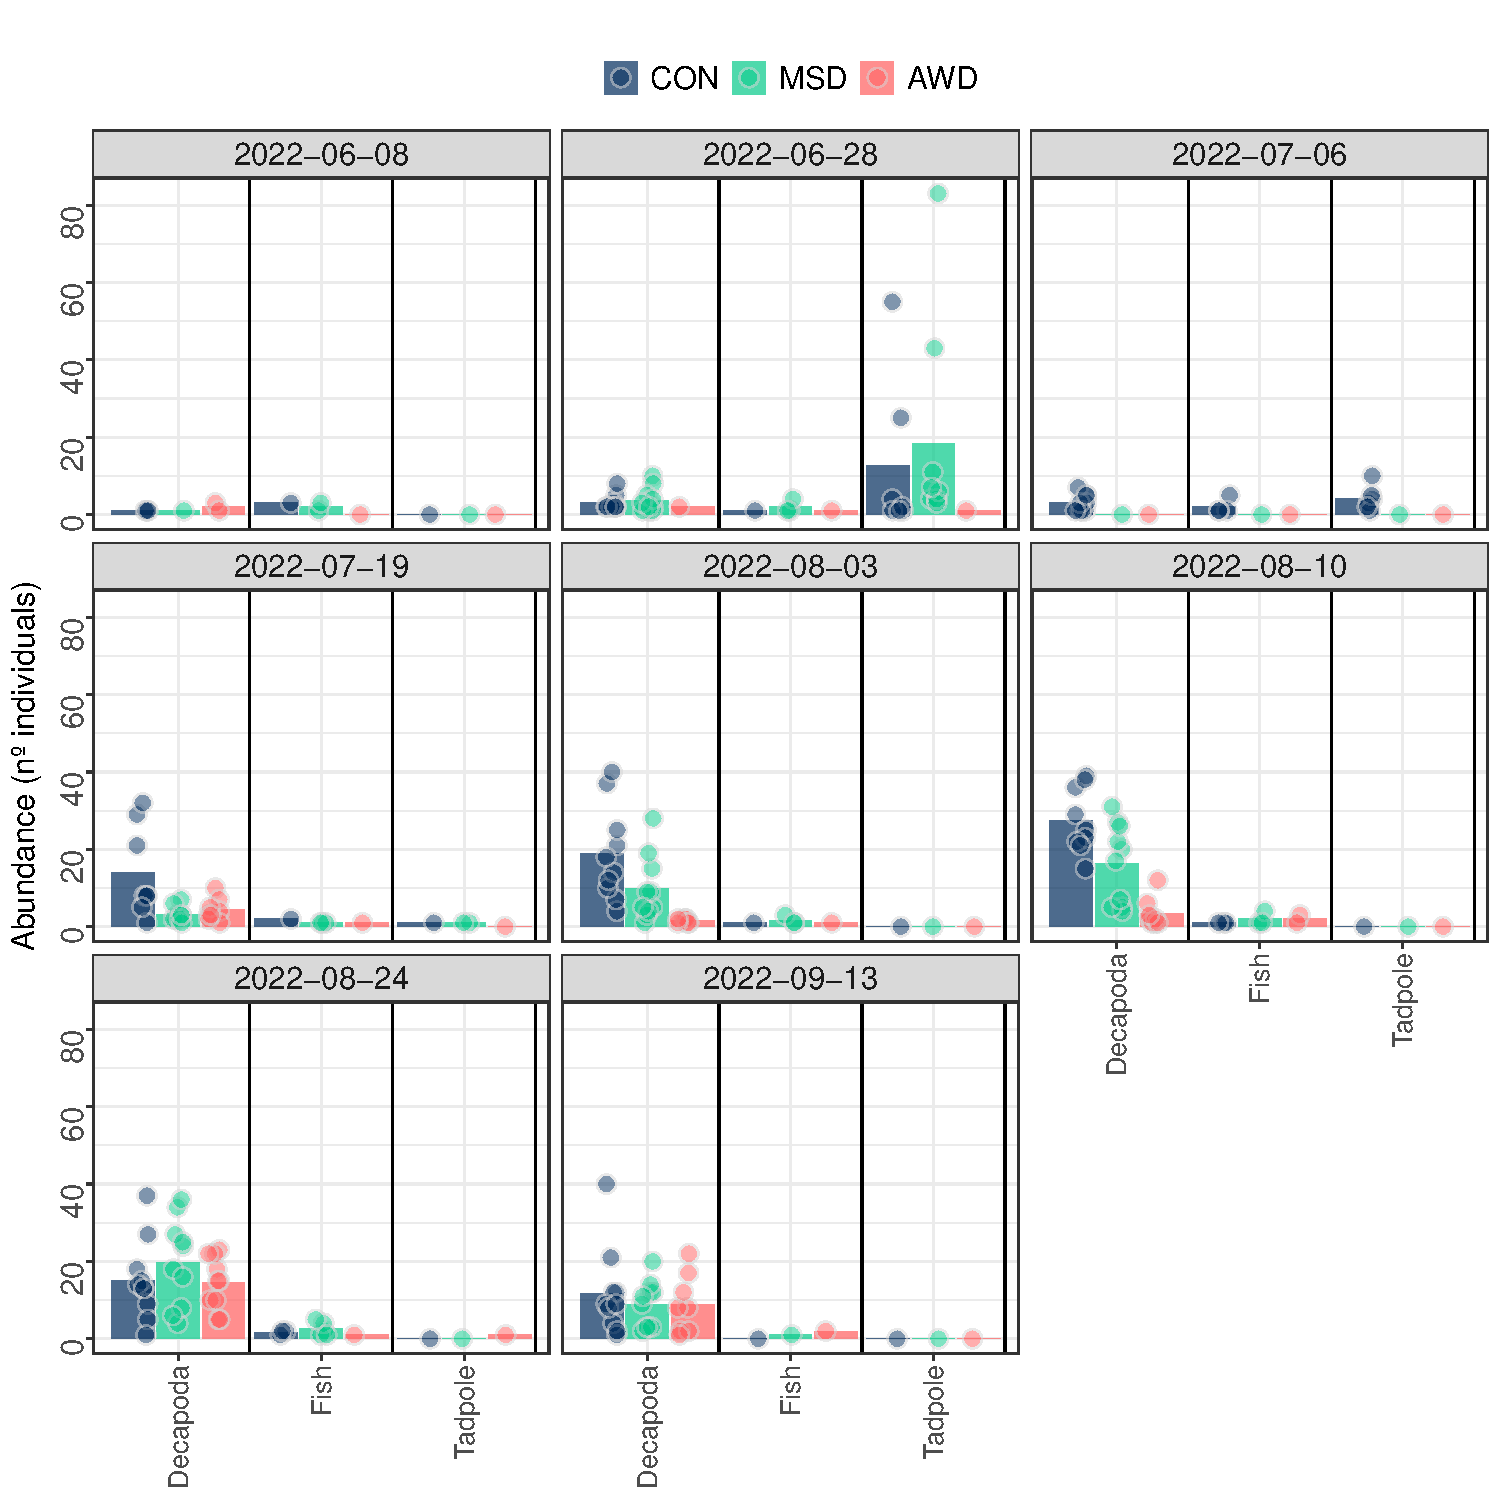
\includegraphics[scale=0.6, center]{Figures/Chapter_1/Abu.div_2022_avg_plots.perDate.pdf}
	\captionof{figure}[Abundance of aquatic communities across the growing season]{Abundance (number of individuals) of sampled aquatic vertebrate (fish and tadpoles) and red swamp crayfish communities for the three water-saving strategies across the rice growing season. Each panel shows observed abundance for a single sampling event (sampling date on top). Bars show mean abundance per irrigation strategy, while points are abundance of individuals per plot. Abbreviations for assessed irrigation strategies stand for: CON = continuous flooding; MSD = mid-season drainage; and AWD = alternate wetting and drying.}   
	\label{Abu_date}
\end{figure*}

% Restore normal figure and table numbering
\renewcommand{\thefigure}{\thechapter.\arabic{figure}}
\setcounter{figure}{0}

\renewcommand{\thetable}{\thechapter.\arabic{table}}
\setcounter{table}{0}



